\chapter{General Relativity}
\label{ch:diff}

Einstein's theory of general relativity allows us to study gravitational physics through understanding how matter curves the spacetime we live within. To understand gravity, we must then understand what it means for a manifold to be curved and the mathematics we use to describe curvature. In this chapter, we introduce the reader to differential geometry, and the mathematical tools we will need while studying black holes. With the ground work of differential geometry, we motivate the postulates of general relativity from looking at the inconsistencies between Newtonian gravity and special relativity. A brief discussion of what it means to solve a gravitational system is given, which is followed by the Lagrangian formulation of general relativity. 

The work contained in this section is based on Wald's `General Relativity' \cite{Wald:106274}, and some old lecture notes written by Reall \cite{Reall:2014gr, Reall:2014bh} from my time at the University of Cambridge. 

\section{Manifolds}
\label{sec:manifolds}

\subsection{Differential manifolds}

If we are to understand gravity through the curvature of spacetime, we must work to understand the spacetime manifold, and how we can perform calculations on it. One of the cornerstones of physics is the application of calculus, which is well defined on the manifold $\Real^n$. The aim of differential geometry is to generalise calculus on spaces which we can only treat as $\Real^n$ locally.

Beginning with a generic manifold $M$, if we consider some small, local patch $\Op \subset M$, we can reasonably approximate $\Op$ as a patch of flat space $\mathcal{U} \subset \Real^n$, \ie if we look at a small enough piece of something curved, it appears flat. If we are able to build our curved manifold from a set of overlapping, flat patches, we can perform calculus over the whole of the manifold; such a manifold is known as a \emph{differential manifold}. The construction of a differential manifold is based on the requirement on correctly gluing together each local piece in a smooth way. 
\begin{defn}
An $n$-dimensional differential manifold is a set $M$ with a collection of subsets $\Op_\alpha$ such that 
\begin{enumerate}[(i)]
	\item Every point in $M$ is in at least one $\Op_\alpha$ \ie the collection $\{\Op_\alpha \}$ covers $M$.
	\item For each $\Op_\alpha$, there is an isomorphic map $ \phi_\alpha: \Op_\alpha \rightarrow \Uc_\alpha$, where $\Uc_\alpha$ is an open subset of $\Real^n$. 
	\item If any two subsets $\Op_\alpha, \Op_\beta$ overlap, there exists a smooth, bijective map $\phi_\beta \circ \phi_\alpha^{-1}$ which maps from $\Uc_\alpha \rightarrow \Uc_\beta$. 
\end{enumerate}
\end{defn}
The maps $\phi_\alpha$ are coordinate systems for the manifold and are sometimes referred to as charts. For the remainder of the thesis, a manifold $M$ is assumed to be a differential manifold, and for this section we assume our manifold $M$ has dimension $n$.


\begin{figure}[!h]
\centering
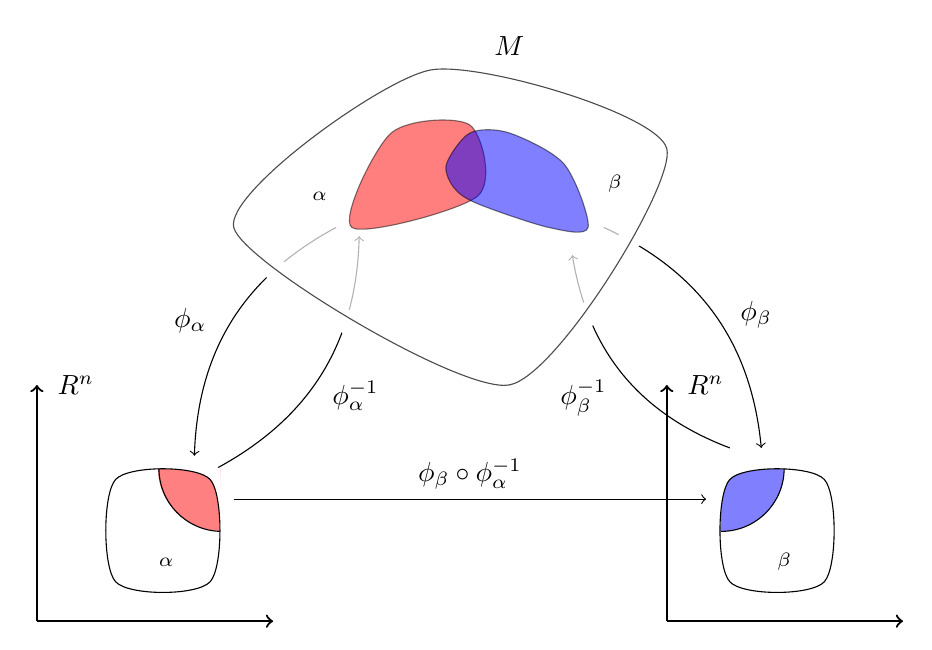
\begin{tikzpicture}

    % Functions i
    \path[->] (0.8, 0) edge [bend right] node[left, xshift=-2mm] {$\phi_\alpha$} (-1, -2.9);
    \draw[white,fill=white] (0.06,-0.57) circle (.15cm);
    \path[->] (-0.7, -3.05) edge [bend right] node [right, yshift=-3mm] {$\phi^{-1}_\alpha$} (1.093, -0.11);
    \draw[white, fill=white] (0.95,-1.2) circle (.15cm);

    % Functions j
    \path[->] (5.8, -2.8) edge [bend left] node[midway, xshift=-5mm, yshift=-3mm] {$\phi^{-1}_\beta$} (3.8, -0.35);
    \draw[white, fill=white] (4,-1.1) circle (.15cm);
    \path[->] (4.2, 0) edge [bend left] node[right, xshift=2mm] {$\phi_\beta$} (6.2, -2.8);
    \draw[white, fill=white] (4.54,-0.12) circle (.15cm);

    % Manifold
    \draw[smooth cycle, tension=0.4, fill=white, opacity=0.7] plot coordinates{(2,2) (-0.5,0) (3,-2) (5,1)} node[opacity=1] at (3,2.3) {$M$};

    % Help lines
    %\draw[help lines] (-3,-6) grid (8,6);

    % Subsets
    % pattern color=red, pattern=north west lines    
    \draw[smooth cycle, fill=red, opacity=0.5] 
        plot coordinates {(1,0) (1.5, 1.2) (2.5,1.3) (2.6, 0.4)} 
        node [label={[label distance=-0.3cm, xshift=-2cm, fill=white, opacity=1]:$\Op_\alpha$}] {};
    \draw[smooth cycle, fill=blue, opacity=0.5] 
        plot coordinates {(4, 0) (3.7, 0.8) (3.0, 1.2) (2.5, 1.2) (2.2, 0.8) (2.3, 0.5) (2.6, 0.3) (3.5, 0.0)} 
        node [label={[label distance=-0.8cm, xshift=0.85cm, yshift=1cm, fill=white, opacity=1]:$\Op_\beta$}] {};

    % First Axis
    \draw[thick, ->] (-3,-5) -- (0, -5) {};
    \draw[thick, ->] (-3,-5) -- (-3, -2) node [label=right:$\mathbb{R}^n$] {};

    % Arrow from i to j
    \draw[->] (-0.5, -3.45) -- node[midway, above]{$\phi_{\beta}\circ \phi_\alpha^{-1}$} (5.5, -3.45);

    % Second Axis
    \draw[thick, ->] (5, -5) -- (8, -5);
    \draw[thick, ->] (5, -5) -- (5, -2) node [label=right:$\mathbb{R}^n$] {};

    % Sets in R^n
	% pattern color=red, pattern=north west lines    
    \draw[white, fill=red!50!white] (-0.67, -3.06) -- +(180:0.8) arc (180:269:0.8);
    \fill[even odd rule, white] [smooth cycle] plot coordinates{(-2, -4.5) (-2, -3.2) (-0.8, -3.2) (-0.8, -4.5)} (-0.67, -3.06) -- +(180:0.8) arc (180:270:0.8);
    \draw[smooth cycle] plot coordinates{(-2, -4.5) (-2, -3.2) (-0.8, -3.2) (-0.8, -4.5)};
    \draw (-1.45, -3.06) arc (180:268:0.8);
    
    \draw[white, fill=blue!50!white] (5.7, -3.07) -- +(-92:0.8) arc (-92:0:0.8);
    \fill[even odd rule, white] [smooth cycle] plot coordinates{(7, -4.5) (7, -3.2) (5.8, -3.2) (5.8, -4.5)} (5.7, -3.06) -- +(-92:0.8) arc (-92:0:0.8);
    \draw[smooth cycle] plot coordinates{(7, -4.5) (7, -3.2) (5.8, -3.2) (5.8, -4.5)};
    \draw (5.69, -3.86) arc (-90:0:0.8);
    
    % labels for R^n
    \node[] at (-1.35, -4.25) {$\Uc_\alpha$};
    \node[] at (6.5, -4.25) {$\Uc_\beta$};
\end{tikzpicture}
\label{fig:diffmanifold}
\caption[Illustration of the mapping for differential manifolds]{An illustration of the mapping $\phi_\beta \circ \phi^{-1}_\alpha$ of two coordinate systems overlapping. A differential manifold requires the mapping between the red and blue sections $\phi_\beta \circ \phi^{-1}_\alpha: \Uc_\alpha \rightarrow \Uc_\beta$ to be smooth.}
\end{figure}



\subsection{Curves, vectors \& tensors}

Both Minkowski and Euclidean manifolds have the structure of a vector space. This means that if we consider some vector, such as the position or velocity of a particle on a flat manifold, we can construct the vector from the manifold itself. For a general manifold, this is not the case. 

For a differential manifold, we recover a vector space by taking a point $p \in M$ and looking at all vectors tangent to this point. This defines a vector space $T_p(M)$ of dimension $n$, known as the \textit{tangent space}. In flat space, the rate of change of a function along a curve at a point $p$ is given as a directional derivative $X_p \cdot (\nabla f)_p$ for a vector $X_p$. We can carry this notion over to differential manifolds by studying the variation of a smooth curve, with some tangent vector $X_p \in T_p(M)$.

\begin{figure}[!h]
\centering
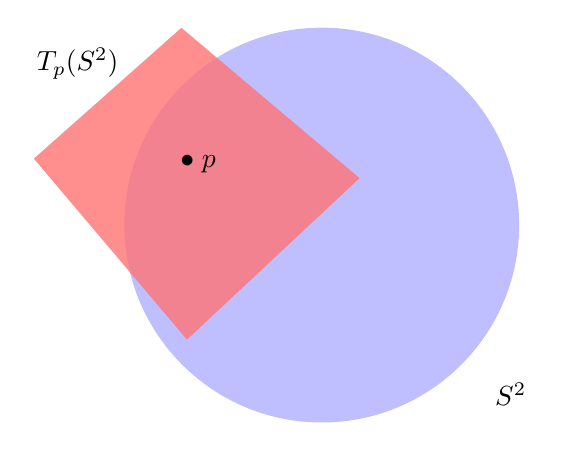
\begin{tikzpicture} % "THE GLOBE" showcase
\tikzfading[name=fade inside,
inner color=transparent!50,
outer color=transparent!50]
\def\R{2.5} % sphere radius
\def\angEl{35} % elevation angle
\filldraw[color=blue!25!white] (0,0) circle (\R);
\fill[red!55!white, opacity=0.8, rotate around={45:(-1.57,0.78)}] (-3.25, -0.7) -- (-3, 2.3) -- (-0.5, 2.15) -- (-0.25, -0.8);

\foreach \t in {-80,-60,...,80} { \DrawLatitudeCircle[\R]{\t} }
\foreach \t in {-5,-35,...,-175} { \DrawLongitudeCircle[\R]{\t} }

\node[] at (-1.57,0.78) {$\bullet \; p$};
\node[] at (-3.1,2.05) {$T_p(S^2)$};
\node[] at (2.4,-2.15) {$S^2$};
\end{tikzpicture}	
\caption[Illustration of the manifold $S^2$ and the tangent space $T_p(S^2)$]{Illustration of the manifold $S^2$ and the tangent space $T_p(S^2)$ at the point $p$ in the manifold.}
\label{fig:spheretangent}
\end{figure}



\begin{defn}
A smooth curve in a differential manifold $M$ is a smooth function mapping $\lambda: I \rightarrow M$, for an open interval $I \in \Real$. We say $\phi_\alpha \circ \lambda$ is a smooth map from $I \rightarrow \Real^n$ for every chart $\phi_\alpha$. 
\end{defn}

\begin{defn}
	Given a smooth curve $\lambda: I \rightarrow M$, the \emph{tangent vector} to $\lambda$ at a point $p$ is a linear map from $M \rightarrow \Real$ defined by:
	\begin{equation*}
		X_p(f) = \diff{}{t} \left(f \circ \lambda \right) .
	\end{equation*}
\end{defn}

Introducing a local coordinate patch $\Uc \subset M$ with coordinates ${x^\mu}$, for a curve $\lambda(t)$ parameterised by $t$, the components of the tangent vector are given by
\begin{equation*}
	X^\mu = \diff{x^\mu}{t}.
\end{equation*}

As well as vectors, which usually are first introduced when studying mechanics, we also work with quantities which map vectors to numbers. These objects are known as \emph{covectors}.
\begin{defn}
	Let $V$ be a finite dimensional, real vector space. The \emph{dual vector space} $V^*$ is the collection of linear maps from $V \rightarrow \Real$.
\end{defn}
When $V$ is finite dimensional, the double dual $V^{**}$ of a vector space is isomorphic to $V$. The dual space to the tangent space $T_p(M)$ is the \emph{cotangent space} $T^*_p(M)$. An element in this space is a covector.

In physics, we not only deal with vectors and covectors but also tensors which are multilinear maps that produce a real number from a set of vectors and covectors. We first contact tensorial objects in mechanics with the energy-momentum tensor, or in electromagnetism with the field strength. In general relativity, the curvature of a spacetime is described using tensors.
\begin{defn}
	A tensor of type $(r,s)$ at the point $p$ is a multilinear map:
	\begin{equation*}
		T: \underbrace{T_p^*(M) \times \ldots \times T_p^*(M)}_{r-\text{times}} \times \underbrace{T_p(M) \times \ldots \times T_p(M)}_{s-\text{times}} \rightarrow \Real.
	\end{equation*}
\end{defn}

The above discussion considered vectors, covectors and tensors defined at a point $p$ in a manifold $M$. When considering physical systems, we are concerned with how these objects vary over the manifold. This leads to the concept of a vector field, where we assign a vector $X_p$ for every $p \in M$. 
\begin{defn}
A \emph{vector field} is a map $X$ which maps a point $p$ in $M$ to a vector $X_p$ in such a way that $X_p$ varies smoothly from point to point. Consider a smooth function $f$, for every point $p \in M$, there exists a function $X(f)$ which maps from the manifold $M \rightarrow \Real$. We say the vector field is smooth if for a smooth function $f$, the function $X(f)$ is also smooth.
\end{defn}
Following this definition, we can think of a covector field as assigning a covector to every point in our manifold and a rank $(r,s)$ tensor field as assigning for each $p \in M$, a $(r,s)$ tensor $T_p$ at $p$.

\begin{defn}
	Given a smooth vector field $X$, an \emph{integral curve} $\gamma$ of $X$, is a curve on $M$ passing through a point $p$ whose tangent everywhere is $X$.
\end{defn}
In a coordinate chart, the existence of an integral curve $\gamma$ parameterised by $t$ can be written as
\begin{equation*}
	\diff{x^\mu}{t} = X^\mu(x(t)), \qquad x^\mu(0) = x^\mu_p.
\end{equation*}
There exists a unique solution to this differential equation, and hence there is an integral curve for all vector fields $X$ through a point $p$.


\subsection{Metric tensor}
\label{sec:metrictensor}
One tensor we will be particularly interested in is the \emph{metric tensor}. Essentially, the metric tensor measures distance on a manifold. We construct the metric tensor as a bilinear scalar function on two vectors such that $g: T_p(M) \times T_p(M) \rightarrow \Real$ which has the following properties:
\begin{defn}
	A \emph{metric tensor} $g$ is a rank (0, 2) tensor which is
	\begin{enumerate}[(i)]
		\item Symmetric: $g(X,Y) = g(Y,X), \quad \forall X,Y \in T_p(M)$
		\item Non-degenerate: $g(X,Y) = 0 \Leftrightarrow Y = 0, \quad \forall X \in T_p(M)$
	\end{enumerate}
\end{defn}
In a coordinate basis, the metric tensor is given by
\begin{equation*}
	g = g_{\mu \nu} dx^\mu \otimes dx^\nu.
\end{equation*}
Commonly the metric tensor is abbreviated to
\begin{equation*}
	ds^2 =  g_{\mu \nu} dx^\mu dx^\nu,
\end{equation*} 
which makes more clear the interpretation of the metric as an \emph{infinitesimal distance squared}. 

The symmetry of the metric tensor ensures that it is possible to introduce a basis that diagonalises the metric. As the metric is non-degenerate, all diagonal elements will be non-zero and so the metric is guaranteed an inverse $g^{-1}$ with components $g^{\mu \nu}$. An \emph{orthonormal basis} can be found such that all diagonal elements of the metric tensor are $\pm 1$. There are many orthonormal bases, but the number of elements which are $+1$ or $-1$ is fixed and the collection of these signs fixes the \emph{signature} of the metric. 

\begin{defn}
	A \emph{pseudo-Riemannian manifold} is a pair $(M, g)$, for a differential manifold $M$ and metric tensor $g$.
\end{defn}

In differential geometry, we are usually concerned with a metric $g$ which is positive-definite. A pseudo-Riemannian manifold with a positive-definite metric $g$ is a \emph{Riemannian manifold}, \ie the metric $g$ has signature $\{++ \ldots + \}$. In general relativity we consider a \emph{spacetime} with the signature $\{-+ \ldots + \}$, such a manifold is known as a \emph{Lorentzian manifold}.\footnote{A $n$-dimensional Lorentzian manifold has a signature $\{\mp, \pm, \ldots, \pm\}$. In relativistic physics --- and this thesis --- the `mostly plus' convention is used. In high-energy physics, the `mostly minus' convention is used where the signature of the metric is $\{+- \ldots - \}$.} For a local patch of a Riemannian (Lorentzian) manifold, the metric tensor is the flat space Euclidean (Minkowski) metric:
\begin{equation*}
	\delta_{\mu \nu} = \fourdiagmat{1}{1}{1}{1}, \qquad \eta_{\mu \nu} = \fourdiagmat{-1}{1}{1}{1} \;.
\end{equation*}

The metric tensor not only acts as a scalar product on two vectors, but also a linear mapping from vectors to covectors. For a pseudo-Riemannian manifold $(M, g)$, given a vector $X^\mu$, we can define a covector $\omega_\mu = g_{\mu \nu} X^\nu$. Similarly, we can define a vector from  a covector $\omega_\nu$ by $X^\mu = g^{\mu \nu} \omega_\nu$.

\begin{defn}
For a Lorentzian manifold $(M,g)$ we classify vectors in the following way. Given a non-zero vector $X \in T_p(M)$, we say a vector is \emph{timelike} if $g(X,X) < 0$, \emph{null} if $g(X,X) = 0$ and \emph{spacelike} if $g(X,X) > 0$.
\end{defn}
This terminology follows to curves. We say that a curve is \emph{timelike} when the tangent vector to the curve is everywhere timelike. The same goes for spacelike or null curves.

\begin{figure}[!h]
\centering

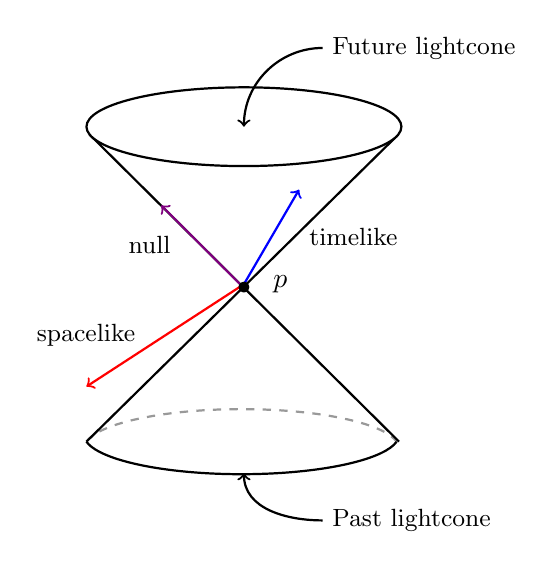
\begin{tikzpicture}
% sides
\draw[thick] (-2,0) -- (1.96,3.9);
\draw[thick] (1.97,0) -- (-1.96,3.9);

% top
\fill[white] (0,4) ellipse (2cm and 0.5cm);
\draw[thick] (0,4) ellipse (2cm and 0.5cm);

% bot
\draw[thick, opacity=0.4, dashed] (-2,0) arc (170:10:2cm and 0.5cm) coordinate[pos=0] (a);
\draw[thick] (-2,0) arc (-170:-10:2cm and 0.5cm) coordinate (b);

% arrows

\draw [->, thick] (1,5) to [out=180,in=90] (0,4);
\node (f)[right] at (1,5) {\small Future lightcone};

\draw [->, thick] (1,-1) to [out=180,in=270] (0,-0.4);
\node (f)[right] at (1,-1) {\small Past lightcone};


\draw[thick, violet, ->] (-0.05,2) -- node[left=0.25cm, black]{\small null} (-1.05,3);
\draw[thick, blue, ->] (0,2) -- node[right=0.35cm, black]{\small timelike} (0.7,3.2);
\draw[thick, red, ->] (0,2) -- node[left=0.25cm, black]{\small spacelike} (-2,0.7);

% point
\node (p1)[right=0.3cm] at (-0.05,2) {$p$};
\node (p2)[] at (0,1.95) {$\bullet$};



\end{tikzpicture}
\caption[Illustration of the Minkowski lightcone]{The lightcone illustrating the causal structure of a point $p$ in a Lorentzian manifold. Null vectors run along the surface of the lightcone, shown in purple. All timelike vectors (blue) lie within the lightcone and spacelike vectors (red) are exterior to the cone.}
\end{figure}


Using the metric, we can now calculate the lengths of timelike and spacelike curves within a manifold. Note that null curves have zero `length'. For a Riemannian manifold $(M,g)$, we can calculate the length of a curve $\lambda: (a,b) \rightarrow M$ with tangent $X$
\begin{equation}
\label{eq:riemlen}
  s = \int^b_a  dt \sqrt{g(X,X)} .
\end{equation}
This may remind the reader of the calculation of a length of a curve in $\Real^n$
\begin{equation*}
  s = \int^b_a  dt \sqrt{ \diff{\mathbf{x}}{t} \cdot \diff{\mathbf{x}}{t} } ,
\end{equation*}
which is simply the case for which $\gmn = \delta_{\mu \nu}$ is the metric for Euclidean space.

For a Lorentzian manifold, the length of a spacelike curve is given by \eq{riemlen}. When the curve $\lambda$ is timelike, the length of the curve is called the \emph{proper time} and is calculated from
\begin{equation}
\label{eq:lorlen}	
  \tau = \int^b_a  du \sqrt{- g(X,X)} .
\end{equation}
When a curve $\lambda$ is parameterised by the proper time, the tangent to the curve is called the \emph{four-velocity} of the curve. The curve is usually denoted by $u^\mu = dx^\mu / d\tau$. Looking infinitesimally at Equation \eq{lorlen}, we have that
\begin{equation*}
	d\tau^2 = - \gmn u^\mu u^\nu \quad \Rightarrow \quad  \gmn u^\mu u^\nu = -1,
\end{equation*} 
and so $u^\mu$ is a unit timelike vector.

Given the notion of length along a curve on a manifold, a natural question is what is the length extremising curve between two points ${p,q} \in M$. In this discussion, we will restrict ourselves to timelike curves, and consider the Euler-Lagrange problem for maximising the proper length of a curve $\lambda(u)$ between two points $p,q \in M$. We write the problem as
\begin{equation*}
	\tau[\lambda] = \int_0^1 du \; L(x(u), \dot{x}(u)), \quad \lambda(0) = p, \; \lambda(1) = q, \quad \dot{x} = \diff{x}{u}.  
\end{equation*}
We can find the extremal curve by ensuring that the functional 
\begin{equation*}
	L = \sqrt{- \gmn(x(u)) \dot{x}^\mu \dot{x}^\nu} ,
\end{equation*}
satisfies Euler-Lagrange's equation
\begin{equation*}
  \diff{}{u} \pardev{L}{\dot{x}^\mu} - \pardev{L}{x^\mu} = 0.
\end{equation*}
We can write this as
\begin{equation*}
  \diff{}{u} \left( \frac{1}{L } g_{\mu \nu} \dot{x}^\nu \right) - \frac{1}{2 L } g_{\nu \rho,\mu} \dot{x}^\nu \dot{x}^\rho = 0.
\end{equation*}
Making a change of parameterisation of the curve from $u$, to the proper time $\tau$, we can rewrite the above equation into the form
\begin{equation*}
  \diff{}{\tau} \left( g_{\mu \nu} \diff{x^\nu}{\tau} \right) - \frac{1}{2} g_{\nu \rho,\mu} \diff{x^\nu}{\tau} \diff{x^\rho}{\tau} = 0,
\end{equation*}
where we have used that
\begin{equation*}
  L^2 = - \gmn \dot{x}^\mu \dot{x}^\nu = \left(\diff{\tau}{u} \right)^2 \quad \Rightarrow \quad \diff{}{u} = L \diff{}{\tau}.
\end{equation*}
Cleaning up the equation and multiplying by the inverse metric, we arrive at the differential equation
\begin{equation}
\label{eq:geodesic}
	\diff{^2 x^\mu}{\tau^2} + \Gamma^\mu_{\nu \rho} \diff{x^\nu}{\tau} \diff{x^\rho}{\tau} = 0.
\end{equation}
Where $\Gamma^{\mu}_{\nu \rho}$ are known as \emph{Christoffel symbols}, given by the expression
\begin{equation}
\label{eq:chs}
   \Gamma^\mu_{\nu \rho} = \half g^{\mu \sigma} (g_{\nu \sigma,\rho} + g_{\rho \sigma,\nu} - g_{\nu \rho,\sigma}).
\end{equation}
We note that the Christoffel symbols are not tensor components, but that their variation is. We will use this later in Section \ref{sec:action}. Equation \eq{geodesic} is the \emph{geodesic equation}. Geodesics themselves will be defined below, after we introduce the notions of a connection on a manifold and parallel transport along a curve.
 

\subsection{Symmetries}

Sometimes we will be interested in mapping from one generic manifold to another, \eg when projecting from a manifold onto a lower-dimensional hypersurface. As with the coordinate basis, we can ensure that this mapping is smooth in the following way.
\begin{defn}
	Let $M$, $N$ be two differential manifolds of dimension $m$ and $n$. A function $\varphi : M \rightarrow N$ is smooth if and only if $\phi_\beta \cdot \varphi \cdot \phi^{-1}_\alpha$ for all coordinate basis $\phi_\alpha$ on $M$ and $\phi_\beta$ on $N$. 
\end{defn}
The mapping $\varphi$ allows us to map objects from one manifold onto another. With a map $\varphi$ we can naturally write a smooth function on $N$, onto $M$ as follows. 
\begin{defn}
	Given a smooth mapping $\varphi : M \rightarrow N$, the \emph{pull-back} of a function $f : N \rightarrow \Real$ is defined as $\phi^\star (f) = f \circ \varphi: M \rightarrow \Real$.
\end{defn}

\begin{figure}[!h]
	\centering
	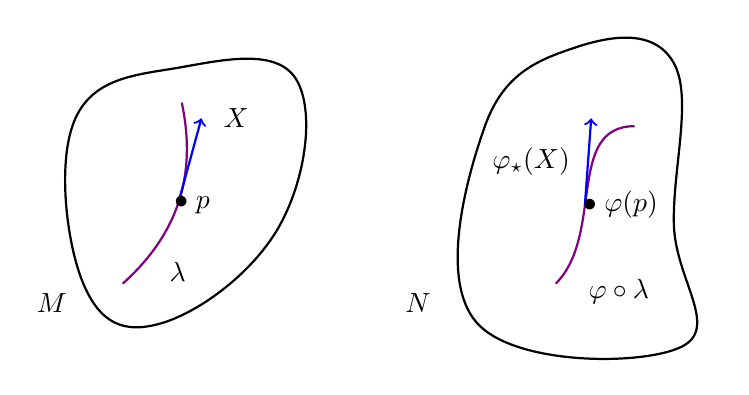
\begin{tikzpicture}
%	helplines
%	\draw[thin] (-5,-4) grid (8,4);
	
	\draw[smooth cycle,tension=.7, thick, xshift=-3cm] plot coordinates{(0,0) (-0.1,2.1) (1.25,2.75) (2.7,2.6) (2.5, 0.75) (1, -0.5)};
	
	
	\draw[smooth cycle,tension=.7, thick, xshift=2cm] plot coordinates{(0,-0.5) (0.1,2) (1.25,3) (2.5,2.8) (2.5, 0.75) (2.6, -0.8)};
	
	\draw[in=180, xshift=3cm, thick, violet] (0,0) to (1,2);
	\draw[bend right, thick, xshift=-3cm, violet] (0.5,0) to (1.25,2.3);
	
	\draw[->, thick, blue] (-1.8,1) -- node[above right=0.3cm, black] {$X$} (-1.5,2.1);
	
	\draw[->, thick, blue] (3.37,1) -- node[left=0.1cm, black] {$\varphi_\star(X)$} (3.45,2.1);
	
	\node (a)[] at (-1.8,0.15) {$\lambda$};
	\node (a)[] at (3.8,-0.1) {$\varphi \circ \lambda$};
	\node (a)[] at (-1.62,1) {$\bullet \; p$};
	\node (a)[] at (3.82,1) {$\bullet \; \varphi(p)$};
	
	\node (a)[] at (-3.4,-0.25) {$M$};
	\node (a)[] at (1.25,-0.25) {$N$};
	

	\end{tikzpicture}
	\caption[Illustration of the mapping between two differential manifolds $M$ and $N$]{Illustration of the mapping between two differential manifolds $M$ and $N$. The smooth map $\varphi$ can push-forward a curve $\lambda$ in $M$ to $N$, where the tangent vector $X \in T_p(M)$ is mapped to the vector $\varphi_\star(X) \in T_{\varphi(p)}$.}
\end{figure}

We can also define a \emph{push-forward}, which naturally takes a curve in $M$ and maps it onto $N$ in the following way.
\begin{defn}
	Given a smooth map $\varphi: M \rightarrow N$, and a point $p \in M$ we can define the \emph{push-forward} of a vector $X^\mu \in T_p (M)$ as the vector $\varphi_\star(X) \in T_{\varphi(p)} (N)$. Given a curve $\lambda$ on $M$ passing through $p$, with tangent $X^\mu \in T_p (M)$, the vector $\varphi_\star(X)$ is the tangent to the curve $\varphi \circ \lambda$ in $N$, at the point $\varphi(p)$.
\end{defn}
The push-forward $\varphi_\star$ can been seen as the total derivative of the map: $\varphi_\star = d\varphi$. Pointwise on the manifold we understand the push-forward as a linear map $\varphi_\star: T_p(M) \rightarrow T_{\varphi(p)} (N)$. Similarly, we understand the pull-back as a pointwise linear mapping from $T^*_{\varphi(p)}(N) \rightarrow T^*_p(M)$. We can extend the action of the pull-back onto a rank $(0,s)$ tensor $S$ as
\begin{equation*}
  (\varphi^\star (S)) (X_1,X_2,\ldots, X_s) = S(\varphi_\star (X_1), \varphi_\star (X_2), \ldots, \varphi_\star (X_s)),
\end{equation*}
for $X_1,X_2,\ldots X_s \in T_p(M)$. Similarly, we extend the action of the push-forward onto a rank $(r,0)$ tensor as
\begin{equation*}
  (\varphi_\star (R)) (\omega_1,\omega_2,\ldots \omega_r) = R(\varphi^\star (\omega_1), \varphi^\star (\omega_2), \ldots, \varphi^\star (\omega_r)),
\end{equation*}
for $\omega_1,\omega_2,\ldots \omega_r \in T^*_p(N)$. However, we can't extended these actions to mixed rank tensors without a further requirement.
\begin{defn}
	We say that the map $\varphi : M \rightarrow N$ is a \emph{diffeomorphism} if and only if it is bijective, smooth and has a smooth inverse.
\end{defn}
If there exists a diffeomorphism $\varphi$ then the two manifolds $M$ and $N$ have the same manifold structure with dim$(M)$ = dim$(N)$. When the mapping is a diffeomorphism, we can use the inverse $\varphi^{-1}$ to extend the pull-back onto a tensor $T$ of mixed rank $(r,s)$ 
\begin{equation*}
\begin{aligned}
	  (\varphi^\star T) (\omega_1,\ldots &\omega_r, X_1,\ldots, X_s) = \\
	  &T ((\varphi^{-1})^\star (\omega_1), \ldots, (\varphi^{-1})^\star (\omega_r), \varphi_\star (X_1), \ldots, \varphi_\star (X_s)). 
\end{aligned}
\end{equation*}
For a diffeomorphism $\varphi$, we have that $\varphi_\star = (\varphi^\star)^{-1}$, and so we need only either the push-forward or pull-back.

Given a diffeomorphism $\varphi: M \rightarrow N$ and a spacetime $(M,g,T)$, the system found after mapping $(N, \varphi_\star (g), \varphi_\star (T))$ is physically indistinguishable from the original system. A tensor $T$ is physically inequivalent to $\tilde{T}$ if and only if there is not a diffeomorphism $\tilde{T} = \varphi^\star(T)$. We then see diffeomorphism invariance as a redundancy in our description of physics in general relativity and so diffeomorphisms are gauge symmetries in general relativity. 

An alternative way to view diffeomorphisms is a mapping from the manifold onto itself, where the mapping $\varphi$ acts as a change of the coordinate basis $\phi_\alpha$. When $\varphi: M \rightarrow M$ is a diffeomorphism and $T$ is a tensor field on $M$, the push-back (pull-forward) allows us to compare $T$ at different points in the manifold. We say that if $\varphi^\star (T) = T$ then $\varphi$ is a symmetry transformation of the tensor field. 

On a manifold $M$, given a vector field $X$, one can construct a diffeomorphism by looking at the map $\phi_t$ which sends a point $p \in M$ along an integral curve a parameter distance $t$. It can be shown that $\phi_t$ is a diffeomorphism \cite{frankel_2011}. Using $\phi_t^\star$, one can compare a tensor along the integral curve of $X$.
\begin{defn}
	The \emph{Lie derivative} of a rank $(r,s)$ tensor at $p \in M$ with respect to a vector $X \in T_p(M)$ is defined by
	\begin{equation}
	\label{eq:liederivative}
		(\La_X T)_p = \lim_{p \rightarrow 0} \frac{(\phi_{-t}^\star (T_p)) - T_p}{t} .
	\end{equation}
\end{defn}
When the diffeomorphism $\phi_t$ is a symmetry of the tensor $T$, then we have
\begin{equation*}
	\La_X T = 0.
\end{equation*}
We will expand on this later, in Section \ref{sec:iso}. The Lie derivative allows us one way to compare tensors at different points in a manifold. In the following section we introduce another way, which leads us naturally to a formal definition of curvature.

\section{Curvature}

We first think about curvature as an experience of some two-dimensional surface embedded within three-dimensional flat space. This type of curvature is mathematically captured by the \emph{extrinsic curvature} and is defined formally in Section \ref{sec:extrinsic}. As an example, we can imagine a rolled up newspaper. The surface of the paper appears `curved' to our eye when viewed from our three-dimensional perspective. However,  allowing the newspaper to unroll, what remains is a flat surface, or approximately $\Real^2$. What we are experiencing is that an object which is flat can be curved into a space of higher dimension. 

There is another type of curvature though, which belongs to a manifold without any notion of embedding. We call this the intrinsic curvature of a manifold. We can compare our newspaper example to the peeling of an orange. In three-dimensional space, the surface of the fruit appears round and in this sense has extrinsic curvature as our rolled newspaper did. However, as we peel the orange we might try to flatten the surface onto the table. What we find that it is impossible to flatten the peel into a good approximation of $\Real^2$. The surface of a sphere in itself is curved.

In general relativity, we are interested in the intrinsic curvature of spacetime. We do not think of our spacetime as being embedded within another manifold, but rather we see gravity manifest itself as the curvature of spacetime itself.  

\subsection{Connections}

\begin{defn}
	A \emph{covariant derivative} $\nabla$ on a manifold $M$ is a mapping from two smooth vector fields $X,Y$ to a smooth vector field $\nabla_X Y$ 
	\begin{equation*}
		\nabla : (X, Y) \longrightarrow \nabla_X Y,
	\end{equation*}
	which obeys the following properties:
	\begin{equation*}
		\begin{aligned}
	\nabla_X(Y + Z) &= \nabla_X Y + \nabla_X Z, \\
	 \nabla_{(fX + gY)} Z &= f\nabla_X Z + g\nabla_Y Z, \\
	 \nabla_X(fY) &= X(f) Y + f\nabla_X Y,
		\end{aligned}
	\end{equation*}
	for all vector fields $X,Y,Z \in T(M)$ and smooth functions $f,g$ on $M$. 
\end{defn}
We note that the action of $\nabla$ on a smooth function $f$ has been defined by: $\nabla_X f = X(f)$. When written in a components, the covariant derivative of a vector field is given by
\begin{equation*}
	\nabla_X Y = X^\mu \nabla_\mu (Y^\rho \partial_\rho) = X^\mu \left(\partial_\mu Y^\rho + \Gamma^{\rho}_{\mu \nu} Y^\nu \right) \partial_\rho,
\end{equation*}
where $\Gamma^{\rho}_{\mu \nu}$ are the \emph{connection components}, we will see later that for a special connection --- the Levi-Civita connection --- the connection components in a coordinate basis are given by the Christoffel symbols \eq{chs}. Using the Leibniz property of the covariant derivative, we can write down the action of $\nabla$ action on a covector $\omega$
\begin{equation*}
	\nabla_X(\omega(Y)) = X(\omega(Y)) = (\nabla_X \omega) Y + \omega (\nabla_X Y),
\end{equation*} 
which shows we should define the action of the connection on a covector as
\begin{equation*}
\begin{aligned}
	&\nabla_X \omega : T(M) \longrightarrow \Real, \\
    &(\nabla_X \omega) (Y) = X(\omega(Y)) -  \omega (\nabla_X Y).
\end{aligned}
\end{equation*}
Written in components
\begin{equation*}
	(\nabla_X \omega) Y = (X(\omega_\mu) - \Gamma^{\rho}_{\mu \nu} \omega_\rho X^\nu) Y^\mu.
\end{equation*}
We can extended this to an arbitrary tensor in the following way
\begin{equation*}
	\nabla_X (T_1 \otimes T_2) = \nabla_X (T_1) \otimes T_2 + T_1 \otimes \nabla_X (T_2) .
\end{equation*} 

\begin{defn}
	A connection is \emph{torsion-free} if the torsion tensor $T(X,Y) = 0$
	\begin{equation*}
		T(X,Y) = \nabla_X Y - \nabla_Y X - [X,Y] .
	\end{equation*}
	In components, this is equivalent to the condition $\Gamma_{[\mu \nu]}^\rho = 0$.
\end{defn}

If given only a manifold, we find that the choice of connection $\nabla$ is not unique, however, with the additional structure of a metric, we can define a unique connection for a pseudo-Riemannian manifold.
\begin{defn}
	Given a pseudo-Riemannian manifold $(M,g)$, there exists a unique torsion-free connection such that $\nabla g = 0$, called the \emph{Levi-Civita} connection.
\end{defn}
We say a connection $\nabla$ is \emph{metric compatible} if $\nabla g = 0$. Deriving the components for the Levi-Civita connection, we find that they are the Christoffel symbols \eq{chs}.

\subsection{Parallel transport}
\label{sec:paralleltransport}

Given a manifold $M$, there is no immediate way of comparing tensors at different points in the manifold. We saw that the Lie derivative allowed us to compare points using diffeomorphisms to compare the value of tensors along integral curves of a vector field. An alternative way is to use a connection $\nabla$ to study how tensors change as we propagate them along some curve $\gamma$ in $M$. We will see that this leads us to the notion of a geodesic; a special curve which describes the path of freely falling objects in general relativity.

\begin{defn}
	Given an integral curve $\gamma$ of a vector field $X$, a tensor $T$ is said to be \emph{parallelly propagated} along $\gamma$ if $\nabla_X T = 0$.
\end{defn}

Taking a vector $X_p$, we can compare it to $X_q$ by parallelly propagating the vector along some curve $\gamma$ which joins the points $p$ and $q$. However, the choice of curve joining two points on a curved manifold is not unique and we find that parallel propagation of a tensor is curve dependent. In other words, picking two distinct curves $\gamma_1$ and $\gamma_2$ the vector $X_p$ will take on two values $X_{q|1}$ and $X_{q|2}$ after parallel propagation. The path dependence of parallel transport is a measure of a manifold's \emph{intrinsic curvature} and is captured formally by the \emph{Riemann curvature tensor}.

\begin{defn}
	The \emph{Riemann curvature tensor} of a connection $\nabla$ is defined by
	\begin{equation}
	\label{eq:riem}
		R(X,Y) Z = \left( \nabla_X \nabla_Y Z - \nabla_Y \nabla_X Z - \nabla_{[X,Y]} Z \right),
	\end{equation}
	for vector fields $X,Y,Z$. 
\end{defn}
Before continuing the discussion of parallel transport, we cover some basic properties of the Riemann tensor. We call a connection \emph{flat} when the Riemann tensor vanishes. In a coordinate basis, the components of the Riemann curvature tensor are given by
\begin{equation}
\label{eq:riemannchs}
   \tensor{R}{^\mu_{\nu \rho \sigma}} = s_2 \left( \partial_\rho \tensor{\Gamma}{^{\mu}_{\nu \sigma}} - \partial_\sigma \tensor{\Gamma}{^{\mu}_{\nu \rho}} + \tensor{\Gamma}{^{\mu}_{\rho \tau}}\tensor{\Gamma}{^{\tau}_{\nu \sigma}} - \tensor{\Gamma}{^{\mu}_{\sigma \tau}}\tensor{\Gamma}{^{\tau}_{\nu \rho}} \right),
\end{equation}
where we have explicitly included the sign $s_2 = \pm 1$ momentarily. In most conventional differential geometry texts, $s_2 = +1$. However, when working with Supergravity, there are other sign conventions and in the work completed in \cite{Gutowski:2019iyo, Gutowski:2020fzb}, we found it most appropriate to make the choice $s_2 = -1$. To maintain consistency throughout this thesis, we will use that $s_2 = -1$ for the remainder of the discussion. As $s_2 = -1$ is unconventional from the differential geometry perspective, we will make appropriate comments throughout this chapter to highlight key differences but refer to Appendix \ref{app:conventions} for a thorough discussion of various signs.

The symmetry of the Riemann tensor means that
\begin{equation*}
	\tensor{R}{^\mu_{\nu (\rho \sigma)}} = 0.
\end{equation*}
For a torsion free connection, the Riemann curvature tensor obeys some other useful relationships. The Christoffel symbols obey $\Gamma^\mu_{[\mu \nu]} = 0$ and the Riemann tensor has the additional property
\begin{equation*}
	\tensor{R}{^\mu_{[\nu \rho \sigma]}} = 0.
\end{equation*}
Contraction of the first or last two indices of the Riemann tensor is zero, but contracting over the first and third gives the \emph{Ricci tensor}, an important tensor in General relativity
\begin{equation}
\label{eq:ric}
  R_{\mu \nu} = \tensor{R}{^{\lambda}_{\mu \lambda \nu}} = -\left( \partial_\lambda \tensor{\Gamma}{^{\lambda}_{\mu \nu}} - \partial_\nu \tensor{\Gamma}{^{\lambda}_{\mu \lambda}} + \tensor{\Gamma}{^{\lambda}_{\lambda \tau}}\tensor{\Gamma}{^{\tau}_{\mu \nu}} - \tensor{\Gamma}{^{\lambda}_{\nu \tau}}\tensor{\Gamma}{^{\tau}_{\mu \lambda}} \right).
\end{equation}
The \emph{Ricci identity}
\begin{equation}
\label{eq:ricid}
	\nabla_\rho \nabla_\sigma X^\mu - \nabla_\sigma \nabla_\rho X^\mu = \tensor{R}{^\mu_{\nu \rho \sigma}} X^\nu,
\end{equation}
allows the interpretation of the Riemann tensor as a measure of the failure for successive operations of the connection to commute. 

The \emph{differential Bianchi identity} is given by
\begin{equation*}
	\nabla_\rho \tensor{R}{^\mu_{\nu \sigma \lambda}} + \nabla_\lambda \tensor{R}{^\mu_{\nu \rho \sigma }} + \nabla_\sigma \tensor{R}{^\mu_{\nu \lambda \rho}} = 0.
\end{equation*}
Contracting first over the indices $(\mu, \rho)$
\begin{equation*}
	\nabla_\mu \tensor{R}{^\mu_{\nu \sigma \lambda}} + \nabla_\lambda R_{\nu \sigma } - \nabla_\sigma R_{\nu \lambda} = 0,
\end{equation*}
then $(\nu,\sigma)$ gives us
\begin{equation*}
	\nabla^\mu G_{\mu \nu} = 0, \qquad G_{\mu \nu} = R_{\mu \nu} - \half R g_{\mu \nu},
\end{equation*}
where $G_{\mu \nu}$ is the \emph{Einstein tensor}, and will appear later as one side of Einstein's equations. When discussing general relativity, we will see that the differential Bianchi identity shows consistency within general relativity for the conservation of the energy-momentum tensor.

So how can we relate parallel transport and the Riemann tensor? Picking some two-dimensional surface $S$ in the manifold $M$, we can construct a small loop that passes through a point $p \in S$ in the following way. We choose coordinates $(t,s)$ on $S$ such that the point $p = (0,0)$. We take vector fields $X = \partial / \partial s$, $Y = \partial / \partial t$ which are linearly independent: $[X,Y] = 0$. We define three more points: $(q,r,u)$ by moving small distances along curves with tangents $X,Y$ such that $q = (\delta s,0)$, $r = (0, \delta t)$ and $y = (\delta s, \delta t)$. Connecting these four points creates a parallelogram $pqur$. 

\begin{figure}[!h]
\centering
\begin{tikzpicture}
\node (I)[circle,fill,inner sep=1.5pt] at (0,0) {};
\node (II)[circle,fill,inner sep=1.5pt] at (2,3) {};
\node (III)[circle,fill,inner sep=1.5pt] at (5,0) {};
\node (IV)[circle,fill,inner sep=1.5pt] at (7,3) {};
\node (Ia) at (-1,0) {$p: (0, 0)$};
\node (IIa) at (1,3) {$r: (0, \delta t)$};
\node (IIIa) at (6,0) {$q: (\delta s, 0)$};
\node (IVa) at (8,3) {$u: (\delta s, \delta t)$};

\draw[black, bend left=14, thick, ->-] (I) to node[midway, left=4pt] {$Y$} (II);
\draw[black, bend left=14, thick, ->-] (III) to node[midway, right=4pt] {$Y$} (IV);
\draw[black, bend left=14, thick, ->-] (I) to node[midway, above=4pt] {$X$} (III);
\draw[black, bend left=14, thick, ->-] (II) to node[midway, above=4pt] {$X$} (IV);

\draw[violet, ->, thick] (0,0) -- (0,1.25);
\draw[blue, ->, thick] (2,3) -- (2.25,3.9);
\draw[blue, ->, thick] (7,3) -- (7.75,3.9);
\draw[red, ->, thick] (5,0) -- (4.8,1.25);
\draw[red, ->, thick] (7,3) -- (6.7,4);

\end{tikzpicture}
\caption[Illustration of parallel propagation]{A vector $V^\mu_p$ (purple) is parallelly propagated along the two curves $pqu$ and $pru$. The resulting vectors $V^\mu_{u|1}$ and $V^\mu_{u|2}$ (red and blue respectively) are not parallel at the point $u$. This is due to the intrinsic curvature of the manifold and is captured by the Riemann curvature tensor.}
\end{figure}

We are now interested in how some vector $V_p \in T_p(M)$ changes as it is parallelly propagated around the loop. We will compare the resulting vectors $V_{u|1}$ and $V_{u|2}$ obtained by parallel propagation along the curves $pqu$ and $pru$ respectively. Along $pq$ we have that $\nabla_X V = 0$ and so
\begin{equation*}
\begin{aligned}
  \diff{V^\mu}{s} &= - \Gamma_{\nu \rho}^\mu V^\nu X^\rho, \\
  \diff{^2 V^\mu}{s^2} &= - \partial_\sigma (\Gamma_{\nu \rho}^\mu V^\nu X^\rho) X^\sigma.
\end{aligned}
\end{equation*}
Using normal coordinates at the point $p$, we have $\Gamma^\mu_{\nu \rho} (p) = 0$ and we can expand the vector field as
\begin{equation}
\label{eq:ppproof1}
	\begin{aligned}
		V^\mu_q &= V^\mu_p + \left(\diff{V^\mu}{s} \right)_p \delta s + \half \left(\diff{^2V^\mu}{s^2} \right)_p \delta s^2 + \Op(\delta s^3) ,\\
		&= V^\mu_p  - \half \left( \partial_\sigma \Gamma_{\nu \rho}^\mu V^\nu X^\rho X^\sigma \right)_p \delta s^2 + \Op(\delta s^3) .
	\end{aligned} 
\end{equation}
We can now look at the parallel transport of $V^\mu_q$ along the curve $qu$. The result can be expanded
\begin{equation*}
\begin{aligned}
	V^\mu_u &= V^\mu_q + \left(\diff{V^\mu}{t} \right)_q \delta t + \half \left(\diff{^2V^\mu}{t^2} \right)_q \delta t^2 + \Op(\delta t^3), \\
	&= V^\mu_q - (\Gamma^\mu_{\nu \rho} V^\nu Y^\rho)_q \delta t - \half \left( \partial_\sigma (\Gamma_{\nu \rho}^\mu V^\nu Y^\rho) Y^\sigma \right)_q \delta t^2 + \Op(\delta t^3), \\
	&= V^\mu_p - \half \left( \partial_\sigma \Gamma^\mu_{\nu \rho} V^\nu \left[ X^\rho X^\sigma \delta s^2 + Y^\rho Y^\sigma \delta t^2 + 2 Y^\rho X^\sigma \delta s \delta t \right] \right)_p + \Op(\delta^3).
\end{aligned}
\end{equation*}
In the third line we have substituted in the results from \eq{ppproof1} and assumed that $\Op(\delta s) = \Op(\delta t) = \Op(\delta)$. The result of parallel propagation for the vector $V^\mu_p$ along the curve $pru$ follows the same steps, and only $X \leftrightarrow Y$ must be swapped in the above equation. We can then look at the difference between these two vectors at $u$:
\begin{equation*}
	\begin{aligned}
		\Delta V^\mu_u \equiv V^\mu_{u |1} - V^\mu_{u |2} &=  \left[ \partial_\sigma \Gamma^\mu_{\nu \rho} V^\nu (Y^\rho X^\sigma - X^\rho Y^\sigma ) \delta s \delta t \right]_p + \Op(\delta^3),\\
		&= [\left(\partial_\rho \Gamma^\mu_{\nu \sigma} - \partial_\sigma \Gamma^\mu_{\nu \rho}  \right) X^\rho Y^\sigma V^\nu]_p + \Op(\delta^3),\\
		&= [\tensor{R}{^\mu_{\nu \rho \sigma}} V^\nu X^\rho Y^\sigma ]_p + \Op(\delta^3), \\
		&= [\tensor{R}{^\mu_{\nu \rho \sigma}} V^\nu X^\rho Y^\sigma ]_u + \Op(\delta^3).
	\end{aligned}
\end{equation*}
Here we have used Equation \eq{riemannchs} and that $\Gamma_{\nu \rho}^\mu(p) = 0$, and in the final line we use that quantities at $p$ and $q$ differ in order $\delta$ and so both the LHS and RHS are tensors at the point $u$. As such, this relationship is basis independent and the Riemann tensor appears as
\begin{equation*}
  \tensor{R}{^\mu_{\nu \rho \sigma}} V^\nu X^c Y^d = \lim_{\delta \rightarrow 0} \frac{\Delta V^\mu_u}{\delta s \delta t}.
\end{equation*}

\subsection{Geodesics}

From the notion of parallel transport, we arrive at the definition of a geodesic. We can think about a geodesic as being a path between two points in a manifold that curves as little as possible. 
\begin{defn}
For a manifold $M$ with connection $\nabla$, a \emph{geodesic} is an integral curve of a vector field $X$ such that $\nabla_X X = \alpha X$, for an arbitrary function $\alpha$. When the function $\alpha = 0$ we say that the geodesic is \emph{affinely parameterised}:
	\begin{equation}
	\label{eq:geod}
	\nabla_X X = 0.
	\end{equation}
	In other words, an affinely parameterised geodesic is the integral curve of the vector field $X$ which is parallelly propagated along itself.	
\end{defn}

Looking at the components, we can write down the geodesic equation in a coordinate basis
\begin{equation}
\label{eq:geocoord}
\begin{aligned}
		X^\nu \nabla_\nu X^\mu &=  X^\nu (\partial_\nu X^\mu + \Gamma^\mu_{\nu \rho} X^\rho), \\
		&= \diff{^2x^\mu}{t^2} + \Gamma^\mu_{\nu \rho} \diff{x^\nu}{t}\diff{x^\rho}{t} .
\end{aligned}
\end{equation}
We can view Equation \eq{geocoord} as a coupled system of $n$ second order differential equations and so from ODE theory, we know that there exists a unique solution given initial values for $x^\mu$ and $d x^\mu / dt$. Therefore, for a given point $p \in M$ and a tangent vector $X^\mu \in T_p(M)$ there is always a unique geodesic through the point $p$ with tangent $X^\mu$.

In Section \ref{sec:metrictensor}, we arrived at the geodesic equation by considering the extremal curve joining two points. However, the existence of a \emph{unique} curve holds only locally. Consider for example the surface of a sphere (see Figure \ref{fig:spheretangent}). The great arcs of a sphere are geodesics and if we take our points $(p,q)$ to be the North and South poles, we find that there is an infinite number of geodesics joining them. This is an example of conjugate points on a Riemannian manifold, for which there exists a one-parameter family of geodesics joining them. We also mention that the length extremising curve is always a geodesic, but not all geodesics are length extremising. Consider again two points on a greats arc of the sphere and the two segments of the great arc which connect them; both of these segments are geodesics. When the points are antipodal, we return to our example of the conjugate points, for all other cases, only one of these geodesics is length minimising.

\subsection{Isometries}
\label{sec:iso}
Earlier, we used diffeomorphisms to define a symmetry of a tensor and saw that this was echoed in the Lie derivative. When the tensor we consider is the metric tensor, we give the symmetry a special name.
\begin{defn}
For a pseudo-Riemannian manifold $(M,g)$ a diffeomorphism $\varphi$ is called an \emph{isometry} when its action on the metric tensor is invariant: $\varphi_\star(g) = g$.
\end{defn}
Given an isometry $\varphi$ and the corresponding vector field $X$, its Lie derivative \eq{liederivative} vanishes: $\La_X g = 0$. We now want to write this in components. The natural action of a Lie derivative on a smooth function $f$ is $\La_X f= X(f)$. In a coordinate basis, we can write the action of a Lie derivative on a vector, covector and $(0,2)$ tensor as:
\begin{equation*}
  \begin{aligned}
    (\La_X Y)^\mu &= [X, Y]^\mu, \\
    (\La_X \omega)_\mu &= X^\nu \nabla_\nu \omega_\mu + \omega_\nu \nabla_\mu X^\nu, \\
   (\La_X T)_{\mu \nu}  &= X^\rho \nabla_\rho T_{\mu \nu} + T_{\mu \rho} \nabla_\nu X^\rho + T_{\rho \nu} \nabla_\mu X^\rho .
  \end{aligned}
\end{equation*}
When we consider an isometry for a pseudo-Riemannian manifold equipped with the Levi-Civita we can simplify the above equation.
\begin{defn}
	Given a one-parameter isometry $\phi_t$ with corresponding vector field $\xi$ on a pseudo-Riemannian manifold $(M,g)$ it follows that $\La_\xi g = 0$. When the connection $\nabla$ is the Levi-Civita connection, isometries are characterised by \emph{Killing's equation}
	\begin{equation}
	\label{eq:killings}
		\nabla_\mu \xi_\nu + \nabla_\nu \xi_\mu = 0.
	\end{equation}
	The vector fields $\xi$ satisfying the above equations are known as \emph{Killing vector fields}. We can interpret a Killing vector field as infinitesimal generators of isometries.
\end{defn}


\begin{lemma}
For a pseudo-Riemannian manifold equipped with the Levi-Civita connection, a Killing vector obeys the identity
\begin{equation}
\label{eq:riekill}
  \nabla_\mu \nabla_\nu \xi_\sigma = \tensor{R}{^\rho_{\mu \nu \sigma}} \xi_\rho.
\end{equation}
\end{lemma}
\begin{proof}
	As the Levi-Civita connection is torsion free, the Killing vector satisfies the Ricci identity \eq{ricid}
	\begin{equation*}
		\nabla_\mu \nabla_\nu \xi_\sigma - \nabla_\nu \nabla_\mu \xi_\sigma = - \tensor{R}{^\rho_{\sigma \mu \nu}} \xi_\rho.
	\end{equation*}
	From the antisymmetry of the Riemann tensor $\tensor{R}{^\mu_{[\nu \rho \sigma]}} = 0$, we can write down that
	\begin{equation*}
		\nabla_{[\mu} \nabla_\nu \xi_{\sigma]} \simeq \tensor{R}{^\mu_{[\sigma \nu \rho]}} \xi^\nu = 0.
	\end{equation*}
	From Killings equation \eq{killings} we have $\nabla_{[\mu} \xi_{\nu]} = 0$, and so antisymmetry in the above equation is equivalent to the cyclic permutation
	\begin{equation*}
		\nabla_\mu \nabla_\nu \xi_\sigma + \nabla_\sigma \nabla_\mu \xi_\nu + \nabla_\nu \nabla_\sigma \xi_\mu = 0,
	\end{equation*}
	which can be rearranged using Killing's equation to give
	\begin{equation*}
	\begin{aligned}
		\nabla_\mu \nabla_\nu \xi_\sigma &= \nabla_\sigma \nabla_\nu \xi_\mu - \nabla_\nu \nabla_\sigma \xi_\mu ,  \\
		&= -\tensor{R}{^\rho_{\mu \sigma \nu}} \xi_\rho, \\
		&= \tensor{R}{^\rho_{\mu \nu \sigma}} \xi_\rho,
	\end{aligned}
	\end{equation*}
	where in the last line, we have used the skew symmetry of the Riemann tensor. 
\end{proof}

\begin{lemma}
	If $\xi^\mu$ is a Killing vector field and $V^\mu$ is tangent to an affinely parameterised geodesic, then the quantity $\xi \cdot V$ is constant along the geodesic.
\end{lemma}

\begin{proof}
Taking the derivative of $\xi \cdot V$ along a geodesic parameterised by $\tau$ we find
\begin{equation*}
  \begin{aligned}
    	\diff{}{\tau} (\xi_\mu V^\mu) &= \nabla_V (\xi_\mu V^\mu) =  V^\nu \nabla_\nu (\xi_\mu V^\mu), \\
    	&= V^\nu V^\mu \nabla_\nu \xi_{\mu} + \xi_{\mu}  V^\nu \nabla_\nu V^\mu = 0.
  \end{aligned}
\end{equation*}
Where in the last line, we lose the first term from the antisymmetry in Killing's equation \eq{killings} and the second term vanishes due to the geodesic equation \eq{geod}.
\end{proof}

This is particularly interesting when we consider the energy-momentum tensor. Given a Killing vector field $\xi^\mu$ and the energy-momentum tensor $T_{\mu \nu}$, we can construct the conserved current $J^\mu = -T_{\mu \nu} \xi^\nu$ such that $\nabla_\mu J^\mu = 0$.

\subsection{Congruences}
\label{sec:congruences}

\begin{defn}
	Given a manifold $M$ and an open set $\mathcal{U} \in M$, a congruence in $\mathcal{U}$ is a family of curves such that exactly one curve passes through each point $p \in \mathcal{U}$. We call this a \emph{geodesic congruence} if the curves are geodesics. 
\end{defn}

Consider a geodesic congruence where all geodesics are either timelike, spacelike or null. When all geodesics of a congruence are of the same type, we can normalise the affine parameter such that the tangent vector $U^\mu$ of the geodesic satisfies $U^2 \in \{-1,1,0\}$ where the three cases are for timelike, spacelike and null geodesics respectively.

In Section \ref{sec:paralleltransport}, we used parallel transport to look at the difference of two vectors as a measure of the curvature of the manifold. We can apply a similar discussion when looking at geodesic congruences, looking at neighbouring geodesic curves and measuring the deviation of their tangent vectors remaining parallel along the curve.

\begin{defn}
A one-parameter family of geodesics is a map: $\gamma : [0,1] \times [0,1] \rightarrow M$ such that
\begin{enumerate}[(i)]
\item For fixed parameter $s$, $\gamma(s,\lambda)$ is a affinely parameterised geodesic .
\item The map $(s,\lambda) \mapsto \gamma(s,\lambda)$ is a smooth bijection.
\end{enumerate}
Together, these two points imply that the family of geodesics span a two-dimensional surface $\Sigma$, parameterised by the coordinates $(s,\lambda)$.
\end{defn}

\begin{figure}[!h]
\centering
\begin{tikzpicture}


\draw[black, bend left=10, thick, -->-] (-2.5,-3) to  (0,1) ;
\draw[black, bend left=10, thick, -->-] (-.2,-3) to (2,1);
\draw[black, bend left=9, thick, -->-] (2.5,-3) to node[at end, yshift=3mm, xshift=1mm] {$s = \text{const.}$} (4,1);

\draw[red, bend right=12, thick, -->-] (-2.7, 0.4) to node[at end, xshift=10mm, black] {$\lambda = \text{const.}$}  (3.3, -1.5) ;
\draw[red, bend right=9, thick, -->-] (-3.1, -1.5) to (3.25, -2.5);

\node[] at (-.25, 0) {$U^\mu$};
\node[] at (1.85, -2.9) {$S^\mu$};

\end{tikzpicture}
\caption[Illustration of two-dimensional hypersurface to aid discussion of congruences]{A sketch of the two-dimensional surface $\Sigma$ spanned by the vectors $U^\mu$ (black) and $S^\mu$ (red). On the surface $\Sigma$, we can use the coordinates $(s,\lambda)$.}
\end{figure}

Let us consider a one-parameter family of geodesics. We refer to the tangent vectors of the geodesics as $U^\mu$ and study the vector $S^\mu$ which is tangent to the curves for constant $\lambda$. Consider the two-dimensional surface $\Sigma$ parameterised by the coordinates $(s,\lambda)$. We can extend these coordinates into a neighbourhood around $\Sigma$ with coordinates $(s,\lambda,\ldots)$ such that
\begin{equation*}
	S = \pardev{}{s}, \quad U = \pardev{}{\lambda}, \quad [S,U] = 0, \qquad U^\nu \nabla_\nu S^\mu = S^\nu \nabla_\nu U^\mu.
\end{equation*}
This relationship allows us to write down
\begin{equation}
\label{eq:geodeviation}
	\nabla_U \nabla_U S = R(U,S) U,
\end{equation}
where we have used that $\nabla_U U = 0$. Equation \eq{geodeviation} is known as the \emph{geodesic deviation equation} and measures the failure for infinitesimally close geodesics within a one-parameter family to have tangent vectors which remain parallel. 
	
We are interested in the geodesic deviation of geodesic congruences. We know that
\begin{equation*}
	\qquad U^\nu \nabla_\nu S^\mu = S^\nu \nabla_\nu U^\mu = \tensor{B}{^\mu_\nu} S^\nu ,
\end{equation*}
where the tensor $\tensor{B}{^\mu_\nu}$ measures the failure of $S^\nu$ to be parallelly transported along the geodesics. For a geodesic congruence where all geodesics are of the same type, we have the additional property that $U^2$ is constant in $\mathcal{U}$, and so we have
\begin{equation*}
	\half \nabla_\mu U^2 = U_\nu \tensor{B}{^\nu_\mu} = 0,
\end{equation*}
and so we can look at 
\begin{equation*}
	U \cdot \nabla (U \cdot S) = \cancel{S^\nu U^\mu \nabla_\mu U_\nu} + U_\nu U^\mu \nabla_\mu S^\nu = U_\nu \tensor{B}{^\nu_\mu} S^\mu = 0,
\end{equation*}
where we have cancelled a term using by that $U^\mu$ is affinely parameterised. We see that $(U \cdot S)$ is constant along the geodesic.

When considering congruences, there is a gauge freedom in how we pick our affine parameter. Even after setting the value of $U^2$, we find we can shift $\lambda$ by a constant value. Scaling $\lambda$ maintains that $U^\mu$ is affinely parametrised, but shifts the displacement vector
\begin{equation*}
	\tilde{\lambda} = \lambda - a(s), \qquad \tilde{S}^\mu = S^\mu + \diff{a}{s} U^\mu.
\end{equation*} 

For timelike and spacelike congruences, we see that the shift in the affine parameter causes a shift in 
\begin{equation*}
	(U \cdot \tilde{S}) = (U \cdot S) + \diff{a}{s} U^2.
\end{equation*}
We can then fix the gauge freedom by picking $\lambda$ such that $(U \cdot S) = 0$. For null congruences where $U^2 = 0$, a shift in $\lambda$ leaves $(U \cdot S)$ invariant and so we need to introduce extra structure to fix the gauge freedom. We delay the further discussion of null congruences until Section \ref{sec:horizonclassify}, where we will look at the properties of them in more detail in the context of trapping regions.


\subsection{Extrinsic curvature}
\label{sec:extrinsic}

Extrinsic curvature is the curvature that we are used to \emph{seeing}. We measure it for lower-dimensional manifolds embedded within our spacetime, \eg the surfaces of the objects we have in front of us can be thought of as embedded within $\Real^3$. We see extrinsic curvature in curves we draw onto pages, or the cylinder we see by rolling up a paper. Before formally defining extrinsic curvature, we must formalise what it means for a surface to be embedded within another.

\begin{defn}
	Let $M$ and $S$ be manifolds of dimension $m$, $s$, with $s < m$. A smooth map $\varphi: M \rightarrow S$ is an \emph{embedding} when $\varphi$ is an injection
		and for any $p \in S$, there is a neighbourhood $\Uc$ such that $\varphi^{-1}: \varphi[\Uc] \rightarrow S$ is smooth.
\end{defn}
\begin{defn}
	Let $M$ and $S$ be manifolds of dimension $m$, $s$, $s <m$. If $\varphi: M \rightarrow S$ is an embedding, we say that $\phi[S]$ is an \emph{embedded submanifold} of $M$. If $s = m-1$ then we say that $S$ is a \emph{hypersurface} denoted by $\Sigma$.
\end{defn}
For a Lorentzian manifold, a hypersurface $\Sigma$ is said to be \emph{timelike}, \emph{spacelike} or \emph{null} corresponding to whether the normal to the surface is everywhere timelike, spacelike or null. 

When working with the action of a gravitational theory, we will be interested in calculating boundary terms for a manifold $M$. The boundary of a manifold $M$ is a hypersurface $\partial M = \Sigma$. In the following discussion, we allow $\Sigma$ to be either timelike or spacelike, with a corresponding unit normal: $n_\mu n^\mu = \epsilon$, where $\epsilon = \pm 1$ for timelike/spacelike $\Sigma$ respectively. The case for null hypersurfaces will be considered later when discussing the geometry of black holes in Section \ref{sec:expansionnullhyper}.

We now have the necessary pieces to define extrinsic curvature. Informally, we can understand the extrinsic curvature as follows. Lets us take a normal vector $n^\mu$ at the point $p \in \Sigma$ and parallelly transport it along a curve $\lambda \in \Sigma$ to the point $q$. The extrinsic curvature measures the failure for this vector to be normal to $\Sigma$ at $q$. 

The first fundamental form, $\gamma_{\mu \nu}$, and can be constructed given the spacetime metric $g_{\mu \nu}$ and the unit normal $n_\mu$ to a hypersurface $\Sigma$. We can understand $\tensor{\gamma}{^\mu_\nu} = \tensor{g}{^\mu_\nu} - \epsilon n^\mu n_\nu$ as either projection operator for tensors in $M$ onto $\Sigma$, or $\gamma_{\mu \nu}$ as the induced metric on $\Sigma$. The second fundamental form is the extrinsic curvature.

Let us consider the parallel transport of a normal vector $N_\mu$ along a curve in $\Sigma$ with a tangent $X^\mu$: $\nabla_X N_\mu = 0$. We can measure the failure of $N_\mu$ remaining normal to $\Sigma$ through considering a second tangent vector: $N \cdot Y \stackrel{?}{=} 0$. We can study how $(N \cdot Y)$ varies along the curve:
\begin{equation*}
	X(N \cdot Y) = X^\mu \nabla_\mu (Y^\nu N_\nu) = N_\nu X^\mu \nabla_\mu Y^\nu.
\end{equation*}
We see that $N \cdot Y = 0$ remains true along the curve iff  $N_\nu X^\mu \nabla_\mu Y^\nu = 0$. This leads to the definition \eq{excurdef} of the extrinsic curvature. By extending our definition of $n_\mu$ in a neighbourhood around a point $p$ in $\Sigma$ into $M$ in an arbitrary way such that $n_\mu$ remains the unit normal, we can write down the extrinsic curvature tensor
\begin{equation}
\label{eq:excurdef}
	K(X,Y) = -s_4 n_\mu \left(\nabla_{X_\parallel} Y_{\parallel} \right)^\mu,
\end{equation}
for vector fields $X,Y$ defined in $M$, and $X_{\parallel}^\mu = \gamma^\mu_\nu X^\nu$ is tangent to $\Sigma$. The sign $s_4 = \pm 1$ is not set through the construction of this tensor. In this thesis, we use that $s_4 = 1$, but note that many other authors use $s_4 = -1$ (see for example Equation (5) in \cite{York1986}). 

\begin{figure}
\centering
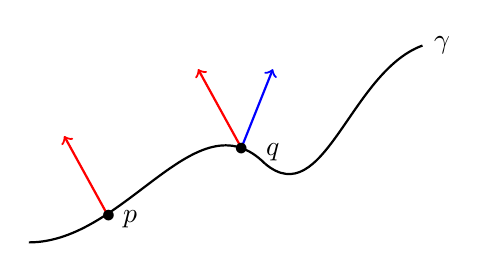
\begin{tikzpicture}[domain=0:5]
  \draw[out=0, thick, black] (0,1) to (3,2);
  \draw[in=200, out=-40, thick, black] (3,2) to (5,3.5);
  \draw[->, red, thick] (1,1.35) -- (0.45,2.35);
  
  \draw[->, red, thick] (2.7,2.2) -- (2.15,3.2);
  \draw[->, blue, thick] (2.7,2.2) -- (3.1,3.2);
  
  \node[] at (1.15,1.3) {$\bullet \; p$};
  \node[] at (2.7,2.18) {$\bullet$};
  \node[] at (3.1,2.15) {$q$};
  \node[] at (5.25,3.5) {$\gamma$};
\end{tikzpicture}
\label{fig:extcurv}
\caption[Illustration of the interpretation of the extrinsic curvature]{The extrinsic curvature measures the failure of a normal to remain normal after parallel transport along a curve. The unit normal at the point $p \in \gamma$ (red) is parallelly propagated along the curve to the point $q$. The extrinsic curvature of $\gamma$ causes the deviation of this vector and the unit normal at the point $q \in \gamma$ (blue).}
\end{figure}
Using that $n_\rho Y^\rho_\parallel = 0$, we can evaluate $K(X,Y)$:
\begin{equation}
			K(X,Y) 
			= - n_\rho X_\parallel^\sigma \nabla_\sigma Y_\parallel^\rho 
			= X_\parallel^\sigma Y_\parallel^\rho \nabla_\rho n_\sigma 
		= (\gamma^\sigma_\mu \gamma^\rho_\nu  \nabla_\rho n_\sigma) X^\mu Y^\nu 
		 = K_{\mu \nu} X^\mu Y^\nu\;.
	\end{equation}
This leads to the expressions
\begin{equation}
\label{eq:extcur0}
	K_{\mu \nu} =  \gamma^\rho_\mu \gamma^\sigma_\nu \nabla_\rho n_\sigma 
	= \nabla_\mu n_\nu - \epsilon n^\rho n_\mu \nabla_\rho n_\nu
	=  \gamma^\rho_\mu \nabla_\rho n_\nu,
\end{equation}
for the extrinsic curvature, where we used $n^\rho \nabla_\mu n_\rho = \frac{1}{2} \nabla_\mu (n^\rho n_\rho)=0$. The boundary can locally be described as the level set of a function $f$. Then $N_\mu = \partial_\mu f$ is a normal vector field, and the corresponding  unit normal vector field $n_\mu$ is hypersurface orthogonal and satisfies the Frobenus integrability condition
\begin{equation}
n_{[\mu} \nabla_\nu n_{\rho]} = 0 \;.
\end{equation}
Contracting this relation with $n^\rho$ it is straightforward to obtain a relation which allows to show that $K_{\mu\nu}$ is symmetric: $K_{\mu \nu} = K_{\nu \mu}$.

In the literature, it is common to see the extrinsic curvature defined through the relation \cite{York1986}
\begin{equation}
\label{eq:extcur2}
	K_{\mu \nu} = \half \La_n \gamma_{\mu \nu}.
\end{equation}
We can verify that this is in the same form as our above definition:
\begin{equation*}
\begin{aligned}
		K_{\mu \nu} &=  \half \La_n \gamma_{\mu \nu}, \\
				&=  \half (n^{c}\nabla_\rho \gamma_{\mu \nu} + \gamma_{\mu \rho} \nabla_\nu n^\rho + \gamma_{\rho \sigma} \nabla_\mu n^\rho), \\
				&=  \half (n^{c}\nabla_\rho (g_{\mu \nu} - \epsilon n_\mu n_\nu) + (g_{\mu \rho} - \epsilon n_\mu n_\rho) \nabla_\nu n^\rho + (g_{\rho \sigma} - \epsilon n_\rho n_\nu) \nabla_\mu n^\rho), \\
				&= \half (\nabla_\mu n_\nu + \nabla_\nu n_\mu - \epsilon n^\rho \nabla_\rho (n_\mu n_\nu)), \\
				&= \nabla_\mu n_\nu - \epsilon n_\mu n^\rho \nabla_\rho n_\nu= K_{\mu \nu}.
\end{aligned}
\end{equation*}
In our calculations, we need the trace of the extrinsic curvature, $K$
\begin{equation}
\label{eq:trext}	
	K = g^{\mu \nu} K_{\mu \nu} = \gamma^{ij} K_{ij},
\end{equation}
where the indices $i,j$ run over the coordinates of $\Sigma$ only. The trace can be calculated from the expression
\begin{equation}
\begin{aligned}
		K &= g^{\mu \nu} K_{\mu \nu} = \half g^{\mu \nu}(\nabla_\mu n_\nu + \nabla_\nu n_\mu - \epsilon n^\rho \nabla_\rho (n_\mu n_\nu)), \\
		&= \half (\nabla_\mu n^{\mu} + \nabla^\mu n_\mu - \cancel{\epsilon n^\rho \nabla_\rho (g^{\mu \nu} n_\mu) n_\nu} ), \\
		&= \nabla_\mu n^\mu \;. \label{K_as_divergence}
\end{aligned}
\end{equation}



\section{General relativity}

\subsection{Motivation}

Einstein's theory of special relativity revolutionised physics. The understanding that our physical laws should be the same in all inertial frames led to developing our concept three-dimensional space, into a four-dimensional spacetime. An event in special relativity is specified by its position within space and time, which we can think of as a point in Minkowski spacetime. Invariance of inertial frames is captured by Lorentz invariance of the tensors on the manifold.

After relativity, it was understood that physical laws should be Lorentz invariant, and so our classical theories would need to be reviewed from this new viewpoint. The constant speed of light bought in new causality constraints, and from this we understood that the instantaneous changes associated with particle interaction would have to be addressed. It was the theory of electromagnetism that led to special relativity, and could be considered as a ready-made theory in regard to being relativistic. However, this was not the case for other physical theories.  

Newton's theory of gravitation was one of these theories. Although very accurate in a low energy limit when the masses were not too large, or the velocities small compared to the speed of light, its formulation is inconsistent with special relativity. The most immediate issue comes from Newton's equation
\begin{equation*}
	\nabla^2 \Phi = 4\pi G \rho,
\end{equation*}
for the gravitational potential $\Phi$ and mass density $\rho$. As a Lorentz transformation will mix together space and time coordinates, there will be inertial frames involving time derivatives, \ie Newton's laws are not invariant between inertial frames. Another way of seeing this same issue can be found from solutions of the potential
\begin{equation*}
  \Phi(t,\mathbf{x}) = -G \int d^3 \mathbf{x} \; \frac{\rho(t,\mathbf{y})}{| \mathbf{x} - \mathbf{y} |}.
\end{equation*}
We see this describes instantaneous response for the potential at $x$ due to an event at $y$, which is incompatible with special relativity.

Despite these issues, Newton's work also gives us a clue on how we might work with relativistic gravity. In Newtonian physics, there are two notions of mass. From Newton's second law, we have the \emph{inertial mass} appearing in the relationship $\mathbf{F} = m_I \mathbf{a}$, and the gravitational mass which determines how a body interacts with the gravitational field: $\mathbf{F} = m_G \mathbf{g}$. The equation for the gravitational field defines both the mass $m_G$ and the acceleration due to gravity $\mathbf{g}$, leading to a scaling ambiguity between them. We fix this by imposing that $m_I = m_G$, which is known as the \emph{weak equivalence principle}. Equality of these two couplings leads to the differential equation
\begin{equation*}
  \ddot{\mathbf{x}} = \mathbf{g}(t,\mathbf{x}).
\end{equation*}
which has a unique solution given a test body's initial position and velocity. Newton's theory doesn't give a \emph{why} to this equivalence, but the Eötvös experiment shows that $m_I / m_G - 1 \simeq \Op(10^{-12})$ \cite{Braginsky1972}. 

It is this equivalence that leads us to the idea of describing gravity as curvature. Let us imagine two bodies which are dramatically different in their composition. The weak equivalence principle states that if these two bodies begin with the same initial position and velocity, they will travel along the same path within spacetime. The independence of a body's composition on the journey they travel through during free fall suggests that the gravitational field is determined by spacetime alone. It is this simple insight that inspired the conjecture that the gravitational force should be seen as a geometric theory of the spacetime.

Newton's equivalence principle is stated for test bodies moving within inertial frames, but how does this extend to areas of physics with additional laws, such as the movement of charged particles? Einstein generalised the equivalence principle in the following way
\begin{defn}
	The \emph{Einstein Equivalence Principle} states that
	\begin{enumerate}[(i)]
		\item The weak equivalence principle is valid.
		\item In a local inertial frame, all non-gravitational experiments will be indistinguishable from the same experiment carried out in a Minkowski inertial frame.
	\end{enumerate}
\end{defn}
We are led to realise that any physical experiment carried out under uniform acceleration would be equivalent to that of one done within a uniform gravitational field. 

So to understand gravity after special relativity, Einstein proposed the theory of general relativity; capturing this equivalence with using geometry. The intrinsic, observer independent nature of spacetime should be described by a spacetime metric, but unlike special relativity, we should not require this to be flat Minkowski space. Einstein prosed that our experience of gravity is captured by the deviation from flatness of the metric of spacetime. Moreover, the curvature of the spacetime metric is caused by the matter within it, and so we relate the curvature of space to a conserved tensor known as the energy-momentum tensor. In essence `\emph{Spacetime tells matter how to move, matter tells spacetime how to curve}' \cite{Misner:1974qy}. We can formalise this paragraph with the postulates of general relativity.
\paragraph{Postulates of General Relativity}
\begin{enumerate}[(i)]
	\item Spacetime is a four-dimensional Lorentzian manifold.
	\item Free particles fall along geodesics of the Levi-Civita connection. Massive particles follow timelike geodesics, massless particles follow null geodesics.
	\item Matter content of a physical system is captured by a $(0,2)$ rank symmetric tensor $T_{\mu \nu}$ called the \emph{energy-momentum} tensor, which is conserved: $\nabla^\mu T_{\mu \nu} = 0$.
	\item The curvature of spacetime is related to the energy-momentum tensor by Einstein's equations
	\begin{equation}
	\label{eq:einstein}
		G_{\mu \nu} \equiv R_{\mu \nu} - \half R g_{\mu \nu} = - 8 \pi G T_{\mu \nu}.
	\end{equation}
\end{enumerate}
The minus sign on the right-hand side comes from our convention $s_3 = -1$ which is explained in more detail within Appendix \ref{app:conventions}. 

We might ask how the form of \eq{einstein} came to be, or whether it could be generalised. When looking for a symmetric tensor of rank $(0,2)$ to be related to the stress-energy tensor, the immediate guess would be the Ricci tensor: $T_{\mu \nu} = c R_{\mu \nu}$, for some constant $c$. However, the conservation of the energy-momentum tensor then implies that $\nabla^\mu R_{\mu \nu} = 0$. This, together with the contracted Bianchi identity implies $\nabla^\mu R = 0$, and hence $\nabla^\mu T = 0$. This would require the energy-momentum tensor to be constant throughout the universe, which obviously isn't the case. Knowing $G_{\mu \nu}$ and the contracted Bianchi identity, we see the Einstein tensor as the natural candidate, but is this the most general solution? The answer comes from Lovelock \cite{Lovelock:1972vz} in the following theorem:
\begin{thm}[Lovelock]
	Let $A_{\mu \nu}$ be a symmetric tensor with the properties
	\begin{itemize}
		\item Metric dependence: $A_{\mu \nu}$ is a function of only $g_{\mu \nu}, \partial_\rho g_{\mu \nu}$ and $\partial_\rho \partial_\sigma g_{\mu \nu}$
		\item Conservation: $\nabla^\mu A_{\mu \nu} = 0$
	\end{itemize}
	Then there exist constants $\alpha, \beta$ such that
	\begin{equation*}
		A_{\mu \nu} = \alpha G_{\mu \nu} + \beta g_{\mu \nu}.
	\end{equation*}
\end{thm}
Lovelock's theorem shows us that Einstein's tensor can be generalised and we can write Einstein's equations as
\begin{equation}
\label{eq:einsteinc}
	R_{\mu \nu} - \half R g_{\mu \nu} + \Lambda g_{\mu \nu} = - 8 \pi G T_{\mu \nu}.
\end{equation}
The constant $\Lambda$ is called the \emph{cosmological constant} and was predicted (and then retracted!!) by Einstein while he was developing his theory of gravity. With $\Lambda \neq 0$, Einstein's equations no longer reduce to Newtonian physics, but if $\Lambda$ is sufficiently small then the deviation is negligible. 

For historical reasons we have kept Newton's constant $(G)$ explicit during the above discussion, while maintaining that the speed of light $c = 1$. We now return to units $G = c = 1$, unless otherwise stated.

\subsection{Solving Einstein's equations}
\label{sec:solvingeinsteinsequations}

Einstein's equations \eq{einstein} describe how spacetime is curved by the matter within it. The solutions to Einstein's equations are given by the metric of the spacetime. The Riemann tensor contains first and second order derivatives of the metric tensor, and so finding solutions of Einstein's equations is equivalent to solving non-linear second order differential equations. The non-linearity of the differential equations separates gravitational solutions from other physical theories \eg the electromagnetic field equations, or Schr\"odinger's equation. 

Due to this non-linearity, exact analytic solutions to Einstein's equations are hard to find, and in general can only be found after making a series of assumptions about the metric tensor. The assumptions for the metric tensor are referred to as the metric ansatz which are formed by writing down the most general metric satisfying a set of assumed isometries. As we saw in Section \ref{sec:iso}, symmetries of the metric tensor manifest as the existence of Killing vector fields of the manifold.

The first non-trivial solution to the vacuum Einstein equations was found by \sch in 1916 \cite{Schwarzschild:1916uq}. To a good approximation, stars and planets are spheres and so a reasonable assumption is that the spacetime geometry containing these massive bodies has the same symmetries as a sphere.
\begin{defn}
A spacetime is \emph{spherically symmetric} if its isometry group contains an SO$(3)$ subgroup with two-sphere orbits. In other words, a manifold is spherically symmetric if it posseses the symmetries of the two-sphere, which has a metric
	\begin{equation*}
	d \Omega^2 = d\theta^2 + \sin^2 \theta d\phi^2		.
	\end{equation*}
\end{defn}
By assuming spherical symmetry of the metric, \sch was able to analytically solve the vacuum equations and describe the geometry of spacetime exterior to a spherically symmetric distribution of uncharged matter. 
\begin{thm}[Birkhoff]
	The unique spherically symmetric solution of the vacuum Einstein equations is the \emph{Schwarzschild solution}. In the coordinates $(t,r,\theta, \phi)$ the \sch metric is given by
	\begin{equation}
	\label{eq:schmet}
	ds^2 = -\left(1 - \frac{2M}{r^2} \right) dt^2 +	\left(1 - \frac{2M}{r^2} \right)^{-1} dr^2 + r^2(d\theta^2 + \sin^2\theta d\phi^2),
	\end{equation}
	where $M$ is a real, positive constant corresponding to the mass of the solution.
\end{thm}

\begin{proof}
	Hawking and Ellis \cite{Hawking:1973uf}.
\end{proof}

The \sch solution is found by assuming spherical symmetry, but there is additional isometry of the spacetime. As the metric \eq{schmet} is time-independent, there is an additional Killing vector: $k^\mu = (\partial_t, 0,0,0)$.
\begin{defn}
	A spacetime is \emph{stationary} is it admits a Killing vector field\footnote{A note for Killing vector notation, we will use $\xi^\mu$ when talking of a generic Killing vector field, and $k^\mu$ when the Killing vector field is also a timelike vector field.} $k^\mu$ that is everywhere timelike: $k^\mu k^\nu g_{\mu \nu} < 0$.
\end{defn}
\begin{defn}
	A spacetime is \emph{static} if it admits a hypersurface-orthogonal Killing vector field. If a spacetime is static, it is also stationary.
\end{defn}
We see that the \sch solution is a static solution and the full isometry group of the metric is $\Real \times \text{SO}(3)$. From Birkhoff's theorem, we realise that the gravitational field exterior to any spherical symmetric distribution of matter is therefore time-independent.

Before moving on, we make a few more comments about the line element \eq{schmet}. We see that the constant $M$ parameterises the solution, and that as we take the limit for $M \rightarrow 0$, the resulting metric is that of Minkowski. The \sch solution is also \emph{asymptotically flat}, which informally can be understood as a spacetime which approaches Minkowski spacetime in the limit $r \rightarrow \infty$. A formal definition for the asymptotic region of a spacetime will be discussed in Section \ref{sec:asymptoticflatness}.

In Section \ref{sec:rnsol}, we derive the \emph{Reissner–Nordstr\"om} solution, a generalisation which allows for the matter distribution to be electromagnetically charged. As a result, we postpone further discussion of the \sch solution and its various properties until later in the thesis.

\subsubsection{Maximally Symmetric Spacetimes}
\label{sec:maximallysymmetric}
To illustrate how assuming the symmetries of the spacetime produces solutions to Einstein's equations, we show how imposing \emph{maximal symmetry} on a spacetime almost uniquely determines the Riemann tensor.

\begin{defn}
	A \emph{maximally symmetric} spacetime is a manifold equipped with the maximum number of linearly independent Killing vector fields.
\end{defn}

\begin{prop}
	For an $n$-dimensional manifold, the maximum number of linearly independent Killing vector fields is given by
	\begin{equation*}
  		\frac{n(n+1)}{2}.
	\end{equation*}
\end{prop}

\begin{proof}
	Given a pseudo-Riemannian manifold $(M,g)$ equipped with the Levi-Civita connection, we are interested in counting the number of linearly independent vector fields which satisfy Killing's equation \eq{killings}. We say that a set of Killing vector fields are \emph{linearly independent} if they are linearly independent as vector fields, \ie for a set of constants $\alpha_i$, the condition
	\begin{equation*}
		\sum_i \alpha_i \xi^i_\mu = 0,
	\end{equation*}
	implies that $\alpha_i = 0$.
	
	From the relationship \eq{riekill}, we see that a Killing vector field is determined uniquely by the data of $\xi_\mu(p)$ and $\nabla_\mu \xi_\nu(p)$ for $p \in M$. We can understand this statement from how \eq{riekill} relates the second derivative of a Killing vector to itself. As a result, given the zeroth and first derivatives of the Killing vector at a point $p \in M$, we can expand and obtain the full solution for Killing vector via the Taylor series. 
	
	For a $n$-dimensional manifold, there can be at most $n$ linearly independent vector fields $\xi_\mu(p)$ at a point $p \in M$. Likewise, there can be at most $n(n-1)/2$ values for $\nabla_\mu \xi_\nu(p)$ due to the antisymmetry of Killing's equation. Combining these results, we obtain that there are 
		\begin{equation*}
  		n + \frac{n(n-1)}{2} = \frac{n(n+1)}{2},
		\end{equation*}
		linearly independent Killing vectors.
\end{proof}

\begin{defn}
	A pseudo-Riemannian manifold $(M,g)$ is \emph{homogeneous} if there exists a group of isometries which acts transitively, \ie any two points $p,q \in M$ can be mapped to each other by a metric preserving symmetry.
\end{defn}

\begin{defn}
\label{def:iso}
	We say that Riemannian (Lorentzian) manifold is \emph{isotropic at a point $p$} if the isotropy group at $p \in M$ acts transitively on the unit sphere (pseudo-sphere) in $T_p(M)$. If a manifold is isotropic for every point in the manifold, it is also homogeneous.
\end{defn}

We take a moment to expand on the second remark in definition \ref{def:iso}. Take a homogenous Riemannian space. Isotropy at a point $p \in M$ can be understood as rotation about the point, \ie the Killing vectors generating the isometry are within $\text{SO}(n)$. Rotating a sphere about a point which is not the sphere's origin acts as a translation of the sphere. If every point in the manifold is invariant under rotation, then it must also be invariant under the translation between two points.

\begin{prop}
	A manifold $M$ is homogeneous and isotropic if and only if it is a maximally symmetric manifold
\end{prop}
\begin{proof}
	S. Kobayashi \cite{kobayashi1967}, S. Gallot \cite{Gallot1987}
\end{proof}

If a maximally symmetric manifold is isotropic at a point $p \in M$, then tensors in the tangent space at that point will be invariant under Lorentz transformations. As the only invariants of the Lorentz group are the Minkowski metric (or products thereof) we can use the symmetries of the Riemann tensor to write the most general form at the point $p$ in the manifold
\begin{equation*}
	R_{\mu \nu \rho \sigma} (p) = f(p) \left( \eta_{\mu \rho} \eta_{\nu \sigma} - \eta_{\mu \sigma} \eta_{\nu \rho} \right). 
\end{equation*}
Allowing the coordinate system to be arbitrary, we replace $\eta_{\mu \nu}$ with a generic metric, but we also know that for all $p \in M$, the spacetime is isotropic, and so we can write down a general expression for the Riemann tensor as
\begin{equation*}
	R_{\mu \nu \rho \sigma} (x) = f(x) \left( g_{\mu \rho} g_{\nu \sigma} - g_{\mu \sigma} g_{\nu \rho} \right) ,
\end{equation*}
for some function $f(x)$. Contracting the Riemann tensor, we find that this function is related to the Ricci scalar
\begin{equation*}
	R_{\mu \nu} = (n - 1) f(x) g_{\mu \nu}, \qquad R = n (n - 1) f(x).
\end{equation*}
We can then write the Riemann tensor for a maximally symmetric spacetime in terms of curvature tensors
\begin{equation*}
	\tensor{R}{_{\mu \nu \rho \sigma}} = \frac{R}{n(n-1)} \left( g_{\mu \rho} g_{\nu \sigma} - g_{\mu \sigma} g_{\nu \rho} \right).
\end{equation*}
Written this way, we see that the Ricci tensor is
\begin{equation}
\label{eq:espace}
	R_{\mu \nu} = \frac1n R g_{\mu \nu}.
\end{equation}
The contracted Bianchi identity gives that
\begin{equation*}
	\nabla^\mu G_{\mu \nu} = \left(\frac1n - \half \right) g_{\nu \sigma} \nabla^\mu R = 0,
\end{equation*} 
where we have used that the Levi-Civita connection is metric compatible. From this, we see that for $n > 2$, the Ricci scalar $R$ must be a constant, and we can write 
\begin{equation*}
	\tensor{R}{_{\mu \nu \rho \sigma}} = \frac{k}{n(n-1)} \left( g_{\mu \rho} g_{\nu \sigma} - g_{\mu \sigma} g_{\nu \rho} \right),
\end{equation*}
for a constant $k$. We do not elaborate on the cases for $n \leq 2$. If a Riemann tensor satisfies the above relationship, it is said to be a \emph{manifold of constant curvature}. As $R$ is constant, from \eq{espace} we see that the Ricci tensor is proportional to the metric tensor and so a maximally symmetric space is also an \emph{Einstein space} \cite{besse1987einstein}.

We thus find that imposing maximally symmetry on our spacetime leads to solutions of Einstein's equations having constant curvature. We can write down Einstein's tensor
\begin{equation*}
	G_{\mu \nu} = R_{\mu \nu} - \half R g_{\mu \nu} + \Lambda g_{\mu \nu} = R \left(\frac1n - \half \right) g_{\mu \nu} + \Lambda g_{\mu \nu},
\end{equation*}
and see that maximally symmetric spacetimes are solutions of the vacuum Einstein equations with a cosmological constant \eq{einsteinc}, where we find
\begin{equation*}
  \Lambda = R \left(\half - \frac1n \right).
\end{equation*}

For a fixed signature, there are only three possible metrics with constant curvature which depend on the sign of $R$. For a Riemannian manifold, a space with $R < 0$ is the sphere, for $R = 0$, the manifold is flat Euclidean space and for $R > 0$, the space is the hyperboloid. For Lorentzian signature, the case for $R = 0$ is flat Lorentzian space, for $R < 0$, the spacetime is called \emph{de Sitter} and the \emph{anti-de Sitter} for $R > 0$. Let us note explicitly that a space of positive curvature has $R < 0$ and a space with negative curvature has $R > 0$. This mismatch of signs comes from our conventions outlined in Appendix \ref{app:conventions} where we explain that a space with positive curvature has sign$(R) = s_1 s_3 = -1$ in our conventions.

The metrics for these maximally symmetric solutions are induced via an embedding of $\Real^{n+1}$. As an example, one can find the  four-dimensional de Sitter metric, beginning with a $(1+4)$-dimensional Lorentzian spacetime
\begin{equation*}
	ds^2 = -dt^2 + dx_1^2 +  \ldots + dx_4^2,
\end{equation*}
from the embedding
\begin{equation*}
	-t^2 + x_1^2 + \ldots x_4^2 = r^2.
\end{equation*}
This can be solved through making the choice
\begin{equation*}
	\begin{aligned}
		t &= r \sinh \tau, \\
		x_1 &= r \cosh \tau \sin \chi \sin \theta \sin \phi, & x_3 &= r \cosh \tau \sin \chi \cos \theta, \\
		x_2 &= r \cosh \tau \sin \chi \sin \theta \cos \phi, & x_4 &= r \cosh \tau \cos \chi.
	\end{aligned}
\end{equation*}
The resulting line element is:
\begin{equation*}
	ds^2 = r^2 \left[- d\tau^2 + \cosh^2 \chi \left(d\chi^2 + \sin^2 \chi \left(d\theta^2 + \sin^2\theta d\phi^2 \right) \right) \right].
\end{equation*}

One can also obtain the metric for these spaces by solving Einstein's equations. As a worked example, let us study three-dimensional Riemannian space. We are interested in solutions to the differential equation
\begin{equation*}
	R_{\mu \nu} = 2k g_{\mu \nu}.
\end{equation*}
The metric describes a homogenous and isotropic manifold, so to start we make an ansatz that the manifold is spherically symmetric with coordinates $(r, \theta, \phi)$
\begin{equation*}
	ds^2 = e^{2F(r)} dr^2 + r^2 (d\theta^2 + \sin^2\theta d\phi^2).
\end{equation*}
From \eq{chs} we can find all non-zero components of the Christoffel symbols
\begin{equation}
   \begin{aligned}
    \tensor{\Gamma}{^{r}_{rr}} &=  \partial_r F(r), & 
    \tensor{\Gamma}{^{r}_{\theta \theta}} &= -re^{-2F}, &
    \tensor{\Gamma}{^{r}_{\phi \phi}} &= -r\sin^2\theta e^{-2F}, &
     & \\
    \tensor{\Gamma}{^{\theta}_{r \theta}} &= \frac{1}{r}, &
    \tensor{\Gamma}{^{\phi}_{r \phi}} &= \frac{1}{r}, &
    \tensor{\Gamma}{^{\theta}_{ \phi \phi}} &= -\cos \theta \sin \theta, &
    \tensor{\Gamma}{^{\phi}_{\theta \phi}} &= \cot \theta.
   \end{aligned}
\end{equation}
Collecting these and inserting them into \eq{ric}, we obtain only three non-zero components of the Ricci tensor
\begin{equation*}
	R_{rr} = -\frac{2 \partial_r F(r)}{r}, \quad R_{\theta \theta} = e^{-2F(r)} \left(1 - e^{2F(r)} - r \partial_r F(r) \right), \quad R_{\phi \phi} = R_{\theta \theta} \sin^2 \theta ,
\end{equation*}
which yields two independent first order differential equations
\begin{gather*}
	2k e^{2F(r)} = -\frac{2 \partial_r F(r)}{r}, \\ 
	2kr^2 = e^{-2F(r)} \left(1 - e^{2F(r)} - r \partial_r F(r) \right).		
\end{gather*}
From the first equation we have
\begin{equation*}
	\partial_r F(r) = -r k e^{2F(r)},
\end{equation*}
which allows us to solve the second equation algebraically, to obtain
\begin{equation*}
	e^{2F(r)} = \frac{1}{1 + k r^2}.
\end{equation*}
Notice that we have found a solution for the metric without solving a differential equation! The metric for a maximally symmetric, three-dimensional Riemannian manifold is given by
\begin{equation*}
	ds^2 = \frac{dr^2}{1 + k r^2}  + r^2 (d\theta^2 + \sin^2\theta d\phi^2).
\end{equation*}
The size of the curvature $k$ can be fixed with a coordinate redefinition, such that there are only three solutions for $k \in \{0,\pm 1\}$. When $k = 0$, we obtain flat space, as we would expect for a solution with zero curvature. For $k = -1$, we obtain the metric on the sphere, and the hyperboloid for $k = 1$.


\subsubsection{Planar Symmetry}

Spherical symmetry is the natural ansatz when looking for solutions to Einstein's equations, but it's not the only assumption we can start with. The main results of this thesis come from considering static solutions which are planar symmetric.

\begin{defn}
A spacetime is \emph{planar symmetric} if its isometry group contains an E$(2)$ subgroup with $\Real^2$ orbits. In other words, a manifold is planar symmetric if it possesses the symmetries of two-dimensional Euclidean space.
\end{defn}

Unlike spherically symmetric solutions, for a four-dimensional spacetime, imposing planar symmetry will not ensure that the spacetime is asymptotically flat. We interpret spacetimes which are not non-asymptotically flat as solutions which have an ever present contribution to the energy-momentum tensor. The de Sitter and anti-de Sitter solutions are the simplest examples of this, where the cosmological constant causes constant curvature throughout the entire spacetime. 

In Chapter \ref{ch:planarem}, the Einstein-Maxwell solution is considered, and by making an ansatz for planar, rather than spherical symmetry, we find dramatic changes in the resulting metric when compared to the Reissner-Nordstr\"om solution derived in Section \ref{sec:rnsol}. The changes between these solutions carries through to the causal structure, the number of horizons and their classification.

If one considers solutions of Einstein's equations in dimensions greater than four, one can obtain asymptotically flat solutions with planar symmetry. In Section \ref{sec:extbranesol}, we will see how these solutions relate to brane solutions of supergravity. Thinking within the context of brane solutions allows the interpretation of planar symmetric solutions in lower dimensions as the dimensional reduction of brane configurations of ten and eleven-dimensional supergravity. Finding solutions with planar symmetry in four dimensions is can then be understood as finding `large brane' solutions of supergravity \cite{Mohaupt:2000gc}.

Imposing spherical symmetry gave the \sch solution to the vacuum Einstein equations, and Birkhoff's theorem showed that this was the unique solution. If the spacetime is assumed to be stationary, the unique planar symmetric solution of the vacuum Einstein's equations is the Taub solution with the corresponding line element \cite{Taub:1951}
\begin{equation*}
	ds^2 = \frac{1}{\sqrt{1 + k z}} \left(-dt^2 + dz^2 \right) + \sqrt{1 + k z} (dx^2 + dy^2).
\end{equation*}
In the limit of $k \rightarrow 0$, we see Taub's line element reduces to the Minkowski solution.  

Another planar symmetric solution comes from the Kasner solutions, which are anisotropic cosmological solutions that depend only on some timelike coordinate $t$. The Kasner solution is described by \cite{Kasner:1921zz}
\begin{equation*}
	ds^2 = -dt^2 +  \sum_{i = 1}^{n-1} t^{p_i} dx_i^2,
\end{equation*}
where the exponents $p_i$ are called the \emph{Kasner exponents}. This metric is an exact solution of Einstein's equations when the Kasner exponents obey
\begin{equation*}
	\sum_{i = 1}^{n-1} p_i = 1, \qquad \sum_{i = 1}^{n-1} p_i^2 = 1.
\end{equation*}
Selecting the constants $p_1 = p_2 = \tfrac{2}{3}$, and $p_3 = - \tfrac{1}{3}$ the above line element can be written as
\begin{equation*}
	ds^2 = - dt^2 + t^{-\frac{1}{3}} dz^2 +  t^{\frac{2}{3}} (dx^2 + dy^2),
\end{equation*} 
and we see that this solution is planar symmetric over the coordinates $(x,y)$.

\subsection{Einstein-Hilbert action}
\label{sec:action}

Einstein's equations describe the dynamic content of general relativity. Given an energy-momentum tensor, one can solve the differential equations $G_{\mu \nu} = - 8\pi T_{\mu \nu}$, and obtain a metric for the spacetime. Despite this, it is still useful to develop a Lagrangian for general relativity. Later, we will use the Lagrangian formulation to construct a partition function for various black hole solutions, which we then use to study the thermodynamics of black holes. More generally, a Lagrangian description for general relativity starts to reach towards the tools and descriptions one would expect for a theory of quantum gravity. If one wanted to calculate the path integral for a gravitational theory, one would need an action and thus a Lagrangian or Hamiltonian of the classical theory. In this section, we keep the various signs $s_i$, which are a collection of conventions one picks when studying general relativity. These are described in more detail in Appendix \ref{app:conventions}. Keeping these signs in our calculations will allow for the comparison of various conventions between the computations of the thesis to external resources.

We would expect our Lagrangian to be of the form:
\begin{equation*}
		S_{EH} = \frac{1}{16 \pi} \int_M d^4 x \sqrt{-g} L ,
\end{equation*} 
for some scalar $L$. An obvious choice would be to use the Ricci scalar $R$, which produces the \emph{Einstein-Hilbert} action 
\begin{equation}
	S_{EH} [g] = \frac{s_1 s_3}{16 \pi} \int_M d^4 x \sqrt{-g} R[g] .
\end{equation} 
This is the action for a vacuum spacetime with no cosmological constant. Note that the dynamical field for the Einstein-Hilbert action is the metric tensor, and so we not only vary the Ricci scalar $R$, but also the volume form itself. 

We now show one can derive Einstein's equations by varying the action
\begin{equation}
\begin{aligned}
\label{eq:ehvar}
		\delta S_{EH} &=  \frac{s_1 s_3}{16 \pi} \int_M d^4 x \; \delta(\sqrt{-g} R)  ,\\
		&=    \frac{s_1 s_3}{16 \pi} \int_M d^4 x ( \delta \sqrt{-g} R + \sqrt{-g} \delta R ) 
\end{aligned}
\end{equation}
To calculate the variation, we look at each term independently. We begin by looking at the variation of the metric determinant. First we write the metric inverse in terms of the determinant and the metric cofactors
\begin{equation*}
	g^{\mu \nu} =  g^{-1} (A^{\mu \nu})^T = g^{-1} A^{\nu \mu} \Rightarrow g = g_{\mu \nu} A^{\mu \nu}.
\end{equation*}
We can then write the variation of the determinant
\begin{equation*}
	\delta g = \pardev{g}{g_{\mu \nu}} \delta g_{\mu \nu} = A^{\mu \nu} \delta g_{\mu \nu} = g g^{\mu \nu} \delta g_{\mu \nu}.
\end{equation*}
Application of the chain rule yields
\begin{equation*}
	\begin{aligned}
\delta \sqrt{-g} &= -\half \frac{\delta g}{\sqrt{-g}}, \\
	 &= -\half \frac{g g^{\mu \nu}}{\sqrt{-g}} \delta g_{\mu \nu}, \\
	&= \half \sqrt{-g} g^{\mu \nu} \delta g_{\mu \nu},  \qquad \qquad g^{\mu \nu} \delta g_{\mu \nu} = - g_{\mu \nu} \delta g^{\mu \nu} ,\\
	&= -\half \sqrt{-g} g_{\mu \nu} \delta g^{\mu \nu}.
	\end{aligned}
\end{equation*} 
We now look at the second term, and calculate the variation of the Ricci scalar. We can break this into a variation of the Ricci tensor and the metric
\begin{equation*}
	\begin{aligned}
		\delta R = \delta g^{\mu \nu} R_{\mu \nu} + g^{\mu \nu} \delta R_{\mu \nu}.
	\end{aligned}
\end{equation*} 
The first term requires no more work. To calculate the Ricci tenor's variation, we have to take a few steps back. The Riemann tensor, written in terms of Christoffel symbols is
\begin{equation*}
\begin{aligned}
		\tensor{R}{^\mu_{\nu \rho \sigma}} &= s_2 \left(\partial_\rho \tensor{\Gamma}{^\mu_{\nu \sigma}} - \partial_\sigma \tensor{\Gamma}{^\mu_{\nu \rho}} +  \tensor{\Gamma}{^\tau_{\nu \sigma}} \tensor{\Gamma}{^\mu_{\tau \rho}} -  \tensor{\Gamma}{^\tau_{\nu \rho}} \tensor{\Gamma}{^\mu_{\tau \sigma}} \right). \\
\end{aligned}
\end{equation*} 
The variation of the Riemann tensor is then given by
\begin{equation*}
	\delta \tensor{R}{^\mu_{\nu \rho \sigma}} = s_2\left(\partial_\rho \delta \tensor{\Gamma}{^\mu_{\nu \sigma}} - \partial_\sigma \delta \tensor{\Gamma}{^\mu_{\nu \rho}}	+  \delta \tensor{\Gamma}{^\tau_{\nu \sigma}} \tensor{\Gamma}{^\mu_{\tau \rho}}  +  \tensor{\Gamma}{^\tau_{\nu \sigma}} \delta \tensor{\Gamma}{^\mu_{\tau \rho}} -  \delta \tensor{\Gamma}{^\tau_{\nu \rho}} \tensor{\Gamma}{^\mu_{\tau \sigma}} - \tensor{\Gamma}{^\tau_{\nu \rho}} \delta \tensor{\Gamma}{^\mu_{\tau \sigma}}  \right).
\end{equation*} 
As mentioned, the Christoffel symbol is not a tensor, but its variation is, and taking the covariant derivative we find that
\begin{equation*}
	\nabla_\sigma (\delta \tensor{\Gamma}{^\mu_{\nu \rho}}) = \partial_ d \delta \tensor{\Gamma}{^\mu_{\nu \rho}} +  \tensor{\Gamma}{^\mu_{\sigma \tau}} \delta \tensor{\Gamma}{^\tau_{\nu \rho}} - \tensor{\Gamma}{^\tau_{\nu \sigma}}\delta \tensor{\Gamma}{^\mu_{\rho \tau}} - \tensor{\Gamma}{^\tau_{\rho \sigma}} \delta \tensor{\Gamma}{^\mu_{\nu \tau}},
\end{equation*}
which can be used to simplify the above expression, given
\begin{equation*}
	\delta \tensor{R}{^\mu_{\nu \rho \sigma}} =   s_2 \left( \nabla_\rho (\delta \tensor{\Gamma}{^\mu_{\nu \sigma}}) - \nabla_\sigma (\delta \tensor{\Gamma}{^\mu_{\nu \rho}}) \right).
\end{equation*}
The variation of the Ricci tensor is then found by contracting the indices:
\begin{equation*}
		s_2 s_3 \delta R_{\mu \nu} = \delta \tensor{R}{^\rho_{\mu \rho \nu}} = s_3 \left( \nabla_\rho (\delta \tensor{\Gamma}{^\rho_{\mu \nu}}) - \nabla_\nu (\delta \tensor{\Gamma}{^\rho_{\rho \mu}}) \right).
\end{equation*} 
The last step is to write out the variation of the Christoffel symbol in terms of variation of the metric. Varying the Christoffel symbol from \eq{chs} results in
\begin{equation*}
	\delta \tensor{\Gamma}{^\rho_{\mu \nu}} = \half \delta g^{\rho \sigma} (\partial_\mu g_{\nu \sigma} + \partial_\nu g_{\mu \sigma} - \partial_\sigma g_{\mu \nu}) + \half g^{\rho \sigma} (\partial_\mu \delta g_{\nu \sigma} + \partial_\nu \delta g_{\mu \sigma} - \partial_\sigma \delta g_{\mu \nu}).
\end{equation*}
The first term can be simplified by writing
\begin{equation*}
	\delta g^{\rho \sigma} = - g^{\rho \sigma} g^{\tau \lambda} \delta g_{\tau \lambda}.
\end{equation*}
To find
\begin{equation*}
	\delta \tensor{\Gamma}{^\rho_{\mu \nu}} = -\tensor{\Gamma}{^\rho_{\mu \nu}} g^{\tau \lambda} \delta g_{\tau \lambda} + \half g^{\rho \sigma} (\partial_\mu \delta g_{\nu \sigma} + \partial_\nu \delta g_{\mu \sigma} - \partial_\sigma \delta g_{\mu \nu}).
\end{equation*}
Then with come careful rearranging of indices we obtain
\begin{equation*}
	\delta \tensor{\Gamma}{^\rho_{\mu \nu}} = \half g^{\rho \sigma} (\nabla_\mu \delta g_{\nu \sigma} + \nabla_\nu \delta g_{\mu \sigma} - \nabla_\sigma \delta g_{\mu \nu}).
\end{equation*}
Finally, contracting the variation with the metric tensor we find
\begin{equation*}
	\begin{aligned}
		g^{\mu \nu} \delta R_{\mu \nu} &= s_3 \left( g^{\mu \nu} \nabla_\rho (\delta \tensor{\Gamma}{^\rho_{\mu \nu}}) - g^{\mu \nu} \nabla_\nu (\delta \tensor{\Gamma}{^\rho_{\rho \mu}}) \right), \\
		&= s_3  \left( \nabla_\rho (g^{\mu \nu}\delta \tensor{\Gamma}{^\rho_{\mu \nu}}) - \nabla_\nu (g^{\mu \nu} \delta \tensor{\Gamma}{^\rho_{\rho \mu}}) \right),\\
		&= s_3 \nabla_\rho (g^{\mu \nu}\delta \tensor{\Gamma}{^\rho_{\mu \nu}} - g^{\mu \rho} \delta \tensor{\Gamma}{^\nu_{ba}}), \\
		&= \frac{s_3}{2} \nabla_\rho (g^{\mu \nu} g^{\rho \sigma} (\nabla_\mu \delta g_{\nu \sigma} + \cancel{\nabla_\nu \delta g_{\mu \sigma}} - \nabla_\sigma \delta g_{\mu \nu}) \\
		&\quad -  g^{\mu \rho}  g^{\nu \sigma} (\nabla_\nu \delta g_{\mu \sigma} + \cancel{\nabla_\mu \delta g_{\nu \sigma}} - \nabla_\sigma \delta g_{\mu \nu}) ), \\
		&= s_3 \nabla^\mu (\nabla^\nu \delta g_{\mu \nu} - g^{\rho \sigma} \nabla_\mu \delta g_{\rho \sigma}).
	\end{aligned}
\end{equation*}
In summary, the two terms varied from the Einstein-Hilbert action are given by
\begin{equation}
	\begin{aligned}
		\delta \sqrt{-g} &= \half \sqrt{-g} g_{\mu \nu} \delta g_{\mu \nu}, \\
		\delta R &= -R^{\mu \nu} \delta g_{\mu \nu} + s_3 \nabla^\mu (\nabla^\nu \delta g_{\mu \nu} - g^{\rho \sigma} \nabla_\mu \delta g_{\rho \sigma}),
	\end{aligned}
\end{equation}
which when substituted into \eq{ehvar}, we find that the variation of the Einstein-Hilbert action is given by
\begin{equation*}
\begin{aligned}
	\delta S_{EH} &= \frac{s_1 s_3}{16 \pi} \int_M d^4 x \; ( \delta \sqrt{-g} R + \sqrt{-g} \delta R ) , \\
	&= \frac{s_1 s_3}{16 \pi} \int_M d^4 x \sqrt{-g} \left(\half g_{\mu \nu} R - R^{\mu \nu} \right) \delta g_{\mu \nu} ,  \\
	& + \frac{s_1}{16 \pi} \int_M d^4 x \sqrt{-g} \nabla^\mu (\nabla^\nu \delta g_{\mu \nu} - g^{\rho \sigma} \nabla_\mu \delta g_{\rho \sigma}) .
\end{aligned}
\end{equation*}
The first term is recognised to be left-hand side Einstein's equations. The second term is a total derivative and for certain boundary conditions can be assumed to be zero. If we do not impose boundary conditions, we can write down the second term as an integral over the boundary $\partial M$ of $M$ where we define the volume form for the hypersurface $\Sigma$ for an \textit{outward} pointed normal vector as:
\begin{equation*}
	d \Sigma_\mu = \epsilon n_\mu \sqrt{|\gamma|} d^3 x.
\end{equation*} 
Using Stoke's theorem:
\begin{equation*}
\begin{aligned}
		\int_M d^4 x \sqrt{-g} \nabla_\mu J^\mu &= \int_M d^4 x \; \partial_\mu (\sqrt{-g} J^\mu) ,\\
		&= \int_{\partial M} J^\mu d \Sigma_\mu,  \\
		&= \int_{\partial M}d^3 x \; \epsilon n^\mu \sqrt{|\gamma|} J_\mu .
\end{aligned}
\end{equation*}
Which when applied to our solution gives:
\begin{equation}
		\delta S_{EH} = \frac{s_1 s_3}{16 \pi} \int_M  d^4x \sqrt{-g} G_{\mu \nu} \delta g^{\mu \nu} + \frac{s_1 \epsilon}{16 \pi} \int_{\partial M}  d^3x \; 1\sqrt{|\gamma|} n^\mu (\nabla^\nu \delta g_{\mu \nu} - g^{\rho \sigma} \nabla_\mu \delta g_{\rho \sigma}) .
\end{equation}
This boundary term is canceled through the addition of the Gibbons-Hawking-York term:
\begin{equation}
	S_{GHY} = \frac{s_1 \epsilon}{8 \pi} \int_{\partial M} d^3 x \; \sqrt{|\gamma|} K,
\end{equation}
where $\gamma$ is the determinant of the induced metric of the hypersurface $\Sigma$ and $K$ is the corresponding trace of the extrinsic curvature, defined in \eq{trext}.
To motivate the inclusion of this term we now consider:
\begin{equation*}
	\delta S_{GHY} = \frac{s_1 \epsilon}{8 \pi} \int_{\partial M}  d^3x \; \delta(\sqrt{|\gamma|} K) = \frac{s_1  \epsilon}{8 \pi} \int_{\partial M}  d^3 x  \left( \delta(\sqrt{|\gamma|})K + \sqrt{|\gamma|} \delta K \right) .
\end{equation*} 
As before, we will solve this variation term by term, beginning with the variation of the unit normal. This is achieved by writing a generic normal covector $N_\mu = \partial_\mu f$ for some function $f$ which is constant on $\Sigma$ and then appropriately normalising to find the unit covector: 
\begin{equation*}
	n_\mu = \frac{\epsilon \partial_\mu f}{ \sqrt{g^{\nu \rho} \partial_\nu f \partial_\rho f }}.
\end{equation*}
Varying this with respect to the spacetime metric we find:
\begin{equation*}
	\begin{aligned}
		\delta n_\mu &= \delta \left( \frac{\epsilon \partial_\mu f}{ \sqrt{g^{\nu \rho} \partial_\nu f \partial_\rho f }} \right), \\
		&= -\half n_\mu \delta g^{\nu \rho} g_{\nu \rho}, \\
		&= \half \epsilon n_\mu n^\nu n^\rho \delta g_{\mu \nu}, \qquad \qquad \epsilon n_\mu n^\rho = g^\rho_\mu - \gamma^\rho_\mu, \\
		&= \frac{1}{2} n^\nu \delta g_{\mu \nu} + c_\nu, \qquad \qquad c_\nu = -\frac{1}{2} \gamma^\rho_\mu \delta g_{\nu \rho} n^\nu ,
	\end{aligned}
\end{equation*}
where $c_\nu$ is orthogonal to $n_\nu$. Before continuing we write down a few useful identities which we will use:
\begin{equation*}
\begin{aligned}
		&n^\mu n^\nu n^\rho = 0, \\
		&\delta n_\mu n^\mu n^\nu = \delta n^\nu.
\end{aligned}
\end{equation*}
Next we can calculate the variation of the induced metric with respect to the spacetime metric:
\begin{equation*}
	\begin{aligned}
		\delta \gamma^{\mu \nu} &= \delta (g^{\mu \nu} - \epsilon n^\mu n^\nu), \\
		&= \delta g^{\mu \nu} - \epsilon \delta n^\mu n^\nu - \epsilon n^\mu \delta n^\nu ,\\
		&= \delta g^{\mu \nu} - \cancel{\epsilon \delta n_\rho n^\rho n^\mu n^\nu} - \cancel{\epsilon n^\mu \delta n_\rho n^\rho n^\nu},	\\	&= \delta g^{\mu \nu} ,
	\end{aligned}
\end{equation*}
and by the same reasoning:
\begin{equation*}
	\delta \gamma^{\mu}_\nu = \delta (\delta^\mu_\nu - \epsilon n^\mu n_\nu) = 0.
\end{equation*}
Using identical methods as for the spacetime metric we find:
\begin{equation*}
	\delta \sqrt{|\gamma|} = -\half \sqrt{|\gamma|} \gamma_{\mu \nu} \delta \gamma^{\mu \nu}.
\end{equation*}
The last thing to calculate is the variation of $K$:
\begin{equation*}
	\begin{aligned}
		\delta K &= \delta (\gamma^{\mu \nu} K_{\mu \nu}) = \delta (\gamma^{\mu \nu} \gamma^\rho_\mu \nabla_\rho n_\nu), \\
		&= \delta \gamma^{\mu \nu} \gamma^\rho_\mu \nabla_{c} n_\nu +  \cancel{\gamma^{\mu \nu} \delta \gamma^\rho_\mu \nabla_{c} n_\nu} +  \gamma^{\mu \nu} \gamma^\rho_\mu \delta(\nabla_{c} n_\nu), \\
		&= \delta \gamma^{\mu \nu} K_{\mu \nu} + \gamma^{\mu \nu} \gamma^\rho_\mu \delta(\partial_\rho n_\nu - \tensor{\Gamma}{^\sigma_{\nu \rho}} n_d) ,\\
		&= \delta \gamma^{\mu \nu} K_{\mu \nu} - \gamma^{\mu \nu} \gamma^\rho_\mu \delta \tensor{\Gamma}{^\sigma_{\nu \rho}} n_d + \gamma^{\mu \nu} \gamma^\rho_\mu \nabla_\rho (\delta n_\nu), \\
		&= \delta K_{(1)} + \delta K_{(2)} + \delta K_{(3)}.
	\end{aligned}
\end{equation*}
To make this easier on the eyes, we now go through this expression term by term. The first term is fine as it is. The second term can be expanded:
\begin{equation*}
\begin{aligned}
		\delta K_{(2)} &= -\gamma^{\mu \nu} \gamma^\rho_\mu \delta \tensor{\Gamma}{^\sigma_{\nu \rho}} n_\sigma ,\\
		&= -\gamma^{\mu \nu} \gamma^\rho_\mu(\half g^{\sigma \tau} (\nabla_\nu \delta g_{\rho \tau} + \nabla_\rho \delta g_{\nu \tau} - \nabla_\tau \delta g_{\nu \rho}))n_\sigma, \\
		&= -\half \gamma^{\mu \nu} \gamma^\rho_\mu n^\tau (\nabla_\nu \delta g_{\rho \tau} + \nabla_\rho \delta g_{\nu \tau} - \nabla_\tau \delta g_{\nu \rho}),
\end{aligned}
\end{equation*}
and the third term can be expanded to
\begin{equation*}
\begin{aligned}
		\delta K_{(3)} &= \gamma^{\mu \nu} \gamma^\rho_\mu \nabla_\rho (\delta n_\nu), \\
		&=  \gamma^{\mu \nu} \gamma^\rho_\mu \nabla_\rho (\frac{1}{2} n^d \delta g_{\nu \sigma} + c_\nu ), \\
		&= \half  \gamma^{\mu \nu} \gamma^\rho_\mu n^d \nabla_\rho \delta g_{\nu \sigma} + \half  \delta g_{\nu \sigma} \gamma^{\mu \nu} \gamma^\rho_\mu \nabla_\rho n^d + \gamma^{\mu \nu} \gamma^\rho_\mu \nabla_\rho c_\nu ,\\
		&= \half  \gamma^{\mu \nu} \gamma^\rho_\mu n^d \nabla_\rho \delta g_{\nu \sigma} + \half  \delta g_{\nu \sigma} K^{\nu \sigma} + D^\nu c_\nu. \\
\end{aligned}
\end{equation*}
Where $D_\mu$ is the covariant derivative projected onto $\Sigma$. Adding these all together we find that:
\begin{equation*}
	\begin{aligned}
		\delta K &= \delta K_{(1)} + \delta K_{(2)} + \delta K_{(3)}, \\
		&= -K^{\mu \nu} \delta \gamma_{\mu \nu} -\half \gamma^{\mu \nu} \gamma^\rho_\mu n^\tau (\nabla_\nu \delta g_{\rho \tau} + \cancel{\nabla_\rho \delta g_{\nu \tau}} - \nabla_\tau \delta g_{\nu \rho}), \\
		&+ \cancel{\half  \gamma^{\mu \nu} \gamma^\rho_\mu n^d \nabla_\rho \delta g_{\nu \sigma}} + \half  \delta g_{\nu \sigma} K^{\nu \sigma} + D^\nu c_\nu, \\
		&= - \half K^{\mu \nu} \delta \gamma_{\mu \nu} -\half \gamma^{\mu \nu} \gamma^\rho_\mu n^d (\nabla_\nu \delta g_{\rho \sigma} - \nabla_\sigma \delta g_{\nu \rho}) + D_\mu c^\mu, \\
		&= - \half K^{\mu \nu} \delta \gamma_{\mu \nu} -\half   \gamma^{\mu \nu} n^\rho (\nabla_\mu \delta g_{\nu \rho} - \nabla_\rho \delta g_{\mu \nu}) + D_\mu c^\mu .
	\end{aligned}
\end{equation*}
Where we have relabelled some dummy indices and cancelled out one term. We are now in a position to accumulate all of these pieces to find that:
\begin{equation*}
\begin{aligned}
		\delta S_{GHY} &= \frac{s_1  \epsilon}{8 \pi} \int_{\partial M}  d^3x \; \delta(\sqrt{|\gamma|} K),  \\
		&= \frac{s_1  \epsilon}{8 \pi} \int_{\partial M}  d^3x \bigg[-\half \sqrt{|\gamma|} \gamma_{\mu \nu} \delta \gamma^{\mu \nu} K  -\half  \sqrt{|\gamma|}  \gamma^{\mu \nu} n^\rho (\nabla_\mu \delta g_{\nu \rho} - \nabla_\rho \delta g_{\mu \nu}) +  \sqrt{|\gamma|} D_\mu c^\mu \bigg] , \\
		&= \frac{s_1 \epsilon}{16 \pi} \int_{\partial M}  d^3x \sqrt{|\gamma|} \; \bigg[ \left(K \gamma_{\mu \nu} - K^{\mu \nu} \right) \delta \gamma^{\mu \nu} -\half   \gamma^{\mu \nu} n^\rho (\nabla_\mu \delta g_{\nu \rho} - \nabla_\rho \delta g_{\mu \nu}) + D_\mu c^\mu \bigg].
\end{aligned}
\end{equation*}
Rewriting for comparison the variation of the Einstein Hilbert action:
\begin{equation*}
		\delta S_{EH} = \frac{s_1 s_3}{16 \pi} \int_M d^4 x \sqrt{-g} G_{\mu \nu} \delta g^{\mu \nu} + \frac{s_1  \epsilon}{16 \pi} \int_{\partial M} d^3 x \sqrt{|\gamma|} n^\mu (\nabla^\nu \delta g_{\mu \nu} - g^{\rho \sigma} \nabla_\mu \delta g_{\rho \sigma}),
\end{equation*}
we see that the inclusion of $S_{GHY}$ will exactly cancel the boundary term which we found in the Einstein-Hilbert variation. This leads us to define a new action:
\begin{equation}
\label{eq:totact}	
\begin{aligned}
		S = \frac{s_1 s_3}{16 \pi} \int_M d^4 x \sqrt{g} R  + \frac{s_1 \epsilon}{8 \pi} \int_{\partial M} d^3 x \sqrt{|\gamma|} K, 
\end{aligned}
\end{equation}
which when varied with respect to the spacetime metric gives a variational principle:
\begin{equation*}
	\delta S = \frac{s_1 s_3}{16 \pi} \int_M d^4 x \sqrt{-g} G_{\mu \nu} \delta g^{\mu \nu}  + \frac{s_1 \epsilon}{16 \pi} \int_{\partial M} d^3x \sqrt{|\gamma|} \bigg[ \left(K \gamma_{\mu \nu} - K^{\mu \nu} \right) \delta \gamma^{\mu \nu} + D_\mu c^\mu \bigg] .
\end{equation*}
We now make a few comments on this action. We know that by Einsteins equations $G_{\mu \nu} = 0$ in a vacuum, and so that term will disappear. It is usually assumed that the metric has zero variation on the boundary $\delta M = \Sigma$. This is to say that $\delta \gamma_{\mu \nu} = 0$. This will remove the second term, and as the last term is a total derivative on the boundary spacetime it is safely ignored. When this boundary condition isn't assumed, we have a further requirement of the extrinsic curvature of the hypersurface:
\begin{equation*}
	\left(K \gamma_{\mu \nu} - K^{\mu \nu} \right) = 0.
\end{equation*} 
This is known as the \textit{Israel Junction Condition}. 

The above discussion assumes that we are working with a vacuum: $T_{\mu \nu} = 0$, but to fully recover Einstein's equations we must include a matter term into our Lagrangian. We allow this to be a generic contribution
\begin{equation*}
	S_m = \int_M d^4x \sqrt{-g} \La_m.
\end{equation*}
The energy-momentum tensor is defined by
\begin{equation*}
	T^{\mu \nu} := s_1 \frac{2}{\sqrt{-g}} \dvar{S_m}{g_{\mu \nu}},
\end{equation*}
and so we find that the variation of the matter term can be written as
\begin{equation*}
	\delta S_m = \frac{s_1}{2} \int_M d^4x \sqrt{-g} T^{\mu \nu} \delta g_{\mu \nu} .
\end{equation*}
Defining the total action as the Einstein-Hilbert term and the matter term together
\begin{equation}
\label{eq:actionatend}
	S = S_{EH} + S_m = \int_M d^4x \sqrt{-g} \left(\frac{s_1 s_3 R}{16\pi} + \La_m \right),
\end{equation}
its variation is found to be
\begin{equation*}
\begin{aligned}
		\delta S &= \frac{s_1 s_3}{16 \pi} \int_M d^4x \sqrt{-g} \left(\half g_{\mu \nu} R - R^{\mu \nu} \right) \delta g_{\mu \nu}  + \frac{s_1}{2} \int_M d^4x\sqrt{-g} T^{\mu \nu} \delta g_{\mu \nu} , \\
		&= \frac{s_1}{16 \pi} \int_M d^4x \sqrt{-g} \left(\half g^{\mu \nu} R - R^{\mu \nu} + s_3 8\pi T^{\mu \nu} \right) \delta g_{\mu \nu} ,
\end{aligned}
\end{equation*}
where for clarity we suppress the boundary conditions. We see that a vanishing variation implies
\begin{equation*}
	R^{\mu \nu} - \half R g^{\mu \nu} = s_3 8\pi T^{\mu \nu},
\end{equation*}
or in other words, Einstein's equations are recovered from varying the action (\ref{eq:actionatend}).
